\ifx\allfiles\undefined
\documentclass[12pt, a4paper,oneside, UTF8]{ctexbook}
\usepackage[dvipsnames]{xcolor}
\usepackage{amsmath}   % 数学公式
\usepackage{amsthm}    % 定理环境
\usepackage{amssymb}   % 更多公式符号
\usepackage{graphicx}  % 插图
%\usepackage{mathrsfs}  % 数学字体
%\usepackage{newtxtext,newtxmath}
%\usepackage{arev}
\usepackage{kmath,kerkis}
\usepackage{newtxtext}
\usepackage{bbm}
\usepackage{enumitem}  % 列表
\usepackage{geometry}  % 页面调整
%\usepackage{unicode-math}
\usepackage[colorlinks,linkcolor=black]{hyperref}

\usepackage{wrapfig}


\usepackage{ulem}	   % 用于更多的下划线格式,
					   % \uline{}下划线,\uuline{}双下划线,\uwave{}下划波浪线,\sout{}中间删除线,\xout{}斜删除线
					   % \dashuline{}下划虚线,\dotuline{}文字底部加点


\graphicspath{ {flg/},{../flg/}, {config/}, {../config/} }  % 配置图形文件检索目录
\linespread{1.5} % 行高

% 页码设置
\geometry{top=25.4mm,bottom=25.4mm,left=20mm,right=20mm,headheight=2.17cm,headsep=4mm,footskip=12mm}

% 设置列表环境的上下间距
\setenumerate[1]{itemsep=5pt,partopsep=0pt,parsep=\parskip,topsep=5pt}
\setitemize[1]{itemsep=5pt,partopsep=0pt,parsep=\parskip,topsep=5pt}
\setdescription{itemsep=5pt,partopsep=0pt,parsep=\parskip,topsep=5pt}

% 定理环境
% ########## 定理环境 start ####################################
\theoremstyle{definition}
\newtheorem{defn}{\indent 定义}[section]

\newtheorem{lemma}{\indent 引理}[section]    % 引理 定理 推论 准则 共用一个编号计数
\newtheorem{thm}[lemma]{\indent 定理}
\newtheorem{corollary}[lemma]{\indent 推论}
\newtheorem{criterion}[lemma]{\indent 准则}

\newtheorem{proposition}{\indent 命题}[section]
\newtheorem{example}{\indent \color{SeaGreen}{例}}[section] % 绿色文字的 例 ,不需要就去除\color{SeaGreen}{}
\newtheorem*{rmk}{\indent \color{red}{注}}

% 两种方式定义中文的 证明 和 解 的环境:
% 缺点:\qedhere 命令将会失效【技术有限,暂时无法解决】
\renewenvironment{proof}{\par\textbf{证明.}\;}{\qed\par}
\newenvironment{solution}{\par{\textbf{解.}}\;}{\qed\par}

% 缺点:\bf 是过时命令,可以用 textb f等替代,但编译会有关于字体的警告,不过不影响使用【技术有限,暂时无法解决】
%\renewcommand{\proofname}{\indent\bf 证明}
%\newenvironment{solution}{\begin{proof}[\indent\bf 解]}{\end{proof}}
% ######### 定理环境 end  #####################################

% ↓↓↓↓↓↓↓↓↓↓↓↓↓↓↓↓↓ 以下是自定义的命令  ↓↓↓↓↓↓↓↓↓↓↓↓↓↓↓↓

% 用于调整表格的高度  使用 \hline\xrowht{25pt}
\newcommand{\xrowht}[2][0]{\addstackgap[.5\dimexpr#2\relax]{\vphantom{#1}}}

% 表格环境内长内容换行
\newcommand{\tabincell}[2]{\begin{tabular}{@{}#1@{}}#2\end{tabular}}

% 使用\linespread{1.5} 之后 cases 环境的行高也会改变,重新定义一个 ca 环境可以自动控制 cases 环境行高
\newenvironment{ca}[1][1]{\linespread{#1} \selectfont \begin{cases}}{\end{cases}}
% 和上面一样
\newenvironment{vx}[1][1]{\linespread{#1} \selectfont \begin{vmatrix}}{\end{vmatrix}}

\def\d{\textup{d}} % 直立体 d 用于微分符号 dx
\def\R{\mathbb{R}} % 实数域
\def\N{\mathbb{N}} % 自然数域
\def\C{\mathbb{C}} % 复数域
\def\Z{\mathbb{Z}} % 整数环
\def\Q{\mathbb{Q}} % 有理数域
\newcommand{\bs}[1]{\boldsymbol{#1}}    % 加粗,常用于向量
\newcommand{\ora}[1]{\overrightarrow{#1}} % 向量

% 数学 平行 符号
\newcommand{\pll}{\kern 0.56em/\kern -0.8em /\kern 0.56em}

% 用于空行\myspace{1} 表示空一行 填 2 表示空两行  
\newcommand{\myspace}[1]{\par\vspace{#1\baselineskip}}

%s.t. 用\st就能打出s.t.
\DeclareMathOperator{\st}{s.t.}

%罗马数字 \rmnum{}是小写罗马数字, \Rmnum{}是大写罗马数字
\makeatletter
\newcommand{\rmnum}[1]{\romannumeral #1}
\newcommand{\Rmnum}[1]{\expandafter@slowromancap\romannumeral #1@}
\makeatother
\begin{document}
	% \title{{\Huge{\textbf{$Real \,\, Analysis$}}}\\
		\Large{\textbf{$Measure \,\, Theory , \,\, Integration , \,\, \& \,\, Hilbert \,\, Spaces$}}\footnote{参考书籍:\\
			\hspace*{4em} \textbf{《$Real \,\, Analysis -- Measure \,\, Theroy, \,\, Integration, \,\, \& \,\, Hilbert \,\, Spaces$》--- $Elias \,\, M. \,\, Stein$} \\
			\hspace*{4em} \textbf{《$Real \,\, Analysis -- Modern \,\, Techniques \,\, and \,\, Their \,\, Applications$》--- $Gerald \,\, B. \,\, Folland$}}}
\author{$-TW-$}
\date{\today}
\maketitle                   % 在单独的标题页上生成一个标题

\thispagestyle{empty}        % 前言页面不使用页码
\begin{center}
	\Huge\textbf{序}
\end{center}


\vspace*{3em}
\begin{center}
	\large{\textbf{天道几何,万品流形先自守;}}\\
	
	\large{\textbf{变分无限,孤心测度有同伦。}}
\end{center}

\vspace*{3em}
\begin{flushright}
	\begin{tabular}{c}
		\today \\ \small{\textbf{长夜伴浪破晓梦,梦晓破浪伴夜长}}
	\end{tabular}
\end{flushright}


\newpage                      % 新的一页
\pagestyle{plain}             % 设置页眉和页脚的排版方式(plain:页眉是空的,页脚只包含一个居中的页码)
\setcounter{page}{1}          % 重新定义页码从第一页开始
\pagenumbering{Roman}         % 使用大写的罗马数字作为页码
\tableofcontents              % 生成目录

\newpage                      % 以下是正文
\pagestyle{plain}
\setcounter{page}{1}          % 使用阿拉伯数字作为页码
\pagenumbering{arabic}
\setcounter{chapter}{0}    % 设置 -1 可作为第零章绪论从第零章开始 
	\else
	\fi
	%  ############################ 正文部分
\chapter{$Measure \,\, Theory$}
\section{$Preliminaries$}
	\begin{defn}\label{def 1.1.1}
		A (closed) \underline{\textbf{rectangle}} $R$ in $\R^d$ is given by of d one-dimensional closed and bounded intervals
		\begin{align}
			R = [a_1 , b_1] \times [a_2 , b_2] \times \cdots \times [a_d , b_d]
		\end{align}
		where $a_j \leq b_j$ are real numbers , $j = 1 , 2 , \cdots , d$. In other word , we have
		\begin{align}
			R = \{ (x_1 , \cdots , x_d) \in \R^d \mid a_j \leq x_j \leq b_j , \,\, \forall j = 1 \sim d \}
		\end{align}
		The \underline{\textbf{volume}} of $R$ is
		\begin{align}
			\left| R \right| = (b_1 - a_1)\cdots(b_d - a_d)
		\end{align}
	\end{defn}

	\vspace*{3em}
	An \textbf{open} rectangle is the product of open intervals , and \underline{\textbf{the interior of the rectangle $R$}} is
	\begin{align}
		(a_1 , b_1) \times (a_2 , b_2) \times \cdots \times (a_d , b_d)
	\end{align}
	Also , a \underline{\textbf{cube}} is a rectangle for which $b_1 - a_1 = \cdots = b_d - a_d$.
	
	\vspace*{3em}
	\begin{defn}\label{def 1.1.2}
		A union of rectangles is said to be \underline{\textbf{almost disjoint}} if the interiors of them are disjoint.
	\end{defn}

	\vspace*{3em}
	\begin{lemma}\label{lemma 1.1.1}
		If a rectangle is the almost disjoint union of finitely many rectangles , say $R = \overset{N}{\underset{k = 1}{\bigcup}}{R_k}$, then
		\begin{align}
			\left| R \right| = \sum_{k = 1}^{N}{\left| R_k \right|}
		\end{align}
	
		\begin{rmk}
			本质上即指的是对于方体的任意的\uwave{\textbf{垂直划分}}可转化为\uwave{\textbf{“十字形”划分}}.
		\end{rmk}
	\end{lemma}

\newpage

	\begin{lemma}\label{lemma 1.1.2}
		If $R , R_1 , \cdots , R_N$ are rectangles , and $R \subset \overset{U}{\underset{k = 1}{\bigcup}}{R_k}$ , then
		\begin{align}
			\left| R \right| \leq \sum_{k = 1}^{N}{\left| R_k \right|}
		\end{align}
		
		\begin{rmk}
			 此即对$Lemma$ \ref{lemma 1.1.1} 的slight modification , 即各方体之间不一定再为almost disjoint.
		\end{rmk}
	\end{lemma}

	\vspace*{3em}
	Now we can give a description of the strcture of open sets in terms of cubes. Begin with the case of $\R$.
	
	\vspace*{2em}
	\begin{thm}\label{thm 1.1.3}
		Every open subset $\mathcal{O}$ of $\R$ can be written uniquely as countable union of disjoint open intervals.
		
		\begin{proof}
			For each $x \in \mathcal{O}$ , let $I_x$ be the largest open interval containing $x$ and contained in $\mathcal{O}$.
			\begin{enumerate}
				\item[$Step \,\, 1 :$]Construct $I_x$:\\
				$\mathcal{O}$ is open $\Rightarrow$ $x$ is contained in some small open interval contained in $\mathcal{O}$.\\
				Let 
				\begin{align}
					a_x &= inf\{ a < x \mid (a , x) \subset \mathcal{O} \} \\
					b_x &= sup\{ b > x \mid (x , b) \subset \mathcal{O} \}
				\end{align}
				Let $I_x = (a_x , b_x)$ , then $\mathcal{O} = \underset{x \in \mathcal{O}}{\bigcup}{I_x}$.
				
				\item[$Step \,\, 2 :$]Suppose $I_x \cap I_y \neq \varnothing$.\\
				$I_x \cup I_y$ is an open interval $\st 
				\begin{cases}
					x \in I_x \cup I_y \\
					I_x \cup I_y \subset \mathcal{O}
				\end{cases}$\\
				Since $I_x$ is maximal , $I_x \cup I_y \subset I_x$. Similarly , $I_x \cup I_y \subset I_y$.\\
				$\Rightarrow \,\, I_x = I_y$ \\
				$\Rightarrow \,\, if \,\, I_x \neq I_y , \,\, then \,\, I_x \cap I_y = \varnothing.$\\
				$\Rightarrow Z = \{ I_x \}_{x \in \mathcal{O}}$ is a disjoint famliy of sets.
				
				\item[$Step \,\, 3 :$]Since every $I_x$ contains at least a $\alpha_x \in \Q$ , construct a map $f$
				\begin{align}
					f : Z &\longrightarrow \Q \\
					I_x &\longmapsto \alpha_x
				\end{align}
				$f$ is an injective. $\Rightarrow \,\, \{ I_x \}_{x \in \mathcal{O}}$ is countable. $\Rightarrow \,\, \mathcal{O} = \overset{\infty}{\underset{j = 1}{\bigcup}}{(a_j , b_j)}$.
			\end{enumerate}
		\end{proof}
	\end{thm}

	\begin{thm}\label{thm 1.1.4}
		Every open set $\mathcal{O}$ of $\R^d$ , $d \geq 1$ , can be written as a countable union of almost disjoint closed cubes.
		
		\vspace*{2em}
		\begin{proof}
			Let 
			\begin{align}
				\mathcal{Q}_k &\coloneqq grid \,\, of \,\, 2^{-k} \Z^d , \,\, k \geq 0 \\
				\underline{A}(\mathcal{O} , k) &\coloneqq \{ Q \in \mathcal{Q}_k \mid Q \subset \mathcal{O} \} \\
				\overline{A}(\mathcal{O} , k) &\coloneqq \{ Q \in \mathcal{Q}_k \mid Q \cap \mathcal{O} \neq \varnothing \}
			\end{align}
			Since $\forall Q \in \underline{A}(\mathcal{O} , k) , \,\, \exists q \in Q^{\circ} , \,\, \st q \in \Q^d , $\\
			According to the Axiom of Choice , $\exists$ the map $f_k : \underline{A}(\mathcal{O} , k) \longrightarrow \Q^d$ , which is an injection.\\
			Hence $\underline{A}(\mathcal{O} , k)$ is countable.\\
			Let
			\begin{align}
				\underline{A}(\mathcal{O}) \coloneqq \bigcup_{k = 1}^{\infty}{\left( \underline{A}(\mathcal{O} , k) \,\, \backslash \,\, \underline{A}(\mathcal{O} , k - 1) \right)} \cup \underline{A}(\mathcal{O} , 0)
			\end{align}
			Then $\underline{A}(\mathcal{O})$ is also countable. Similarly define $\overline{A}(\mathcal{O})$.\\
			$\forall x \in \mathcal{O}$ , let $\delta_x \coloneqq inf \{ \left| y - x \right| \mid y \notin \mathcal{O} \}$. Since $\mathcal{O}$ is open , $\Rightarrow \,\, \delta_x > 0$.
			\begin{align}
				&\exists N_x \in \N , \,\, \st 2^{-k}\sqrt{d} \leq \frac{\delta_x}{2} < \delta_x , \forall k \geq N_x \\
				&\Rightarrow \forall Q \in \overline{A}(\mathcal{O} , N_x) , \,\, \st \left| s - t \right| \leq 2^{-N_x}\sqrt{d} < \delta_x , \forall s , t \in Q \\
				&\Rightarrow Since \,\, \mathcal{O} \subset \overline{A}(\mathcal{O}) , \,\, \exists Q_x \in \overline{A}(\mathcal{O} , N_x) \subset \overline{A}(\mathcal{O}) , \,\, \st x \in Q_x  \\
				&\Rightarrow x \in Q_x \subset \mathcal{O} \\
				&\Rightarrow x \in Q_x \in \underline{A}(\mathcal{O} , N_x) \subset \underline{A}(\mathcal{O}) \\
				&\Rightarrow \mathcal{O} \subset \underline{A}(\mathcal{O})
			\end{align}
			Obviously $\underline{A}(\mathcal{O}) \subset \mathcal{O}$ , so 
			\begin{align}
				\mathcal{O} = \underline{A}(\mathcal{O}) = \bigcup_{k = 1}^{\infty}{\left( \underline{A}(\mathcal{O} , k) \,\, \backslash \,\, \underline{A}(\mathcal{O} , k - 1) \right)} \cup \underline{A}(\mathcal{O} , 0)
			\end{align}
			which is a countable union of almost disjoint closed cubes.
		\end{proof}
	\end{thm}

\newpage
\section{$The \,\, Exterior \,\, Measure$}
\paragraph{$Definition$}
	The exterior measure attempts to describe the volume of a set $E$ by approximating it from the outside.\\ Loosely speaking , the exterior measure $m_{*}$ assigns to \textbf{any subset of $\R^d$} a first notion of size.
	\begin{defn}\label{def 1.2.1}
		If $E$ is a subset of $\R^d$ , the \underline{\textbf{exterior measure}} of $E$ is
		\begin{align}
			m_{*}(E) \coloneqq \inf{ \left\{ \sum_{j = 1}^{\infty}{\left| Q_j \right| \,\, \Big| \,\, E \subset \bigcup_{j = 1}^{\infty}{Q_j} , \,\, Q_j \,\, is \,\, a \,\, closed \,\, cube } \right\} }
		\end{align}
	
		\begin{rmk}
			\begin{itemize}
				\item \textbf{Well definition:}  $\forall E \subset \R^d , \,\, E \subset \overset{\infty}{\underset{n = 1}{\bigcup}}{Q_n} , \,\, Q_n = [-n , n]^d \subset \R^d$ , which means $m_{*}$ can be defined on every subset of $\R^d$.
				
				\item It is immediate from the definition that:\\
				For every $\epsilon > 0$ , there exists a covering $E \subset \overset{\infty}{\underset{j = 1}{\bigcup}}{Q_j} , \,\, \st$
				\begin{align}
					\sum_{j = 1}^{\infty}{m_{*}(Q_j)} \leq m_{*}(E) + \epsilon
				\end{align}
				
				\item It is important to note that it would \textbf{not suffice} to allow \textbf{finite sums} in the definition of $m_{*}(E)$. If one considered only coverings of $E$ by finite unions of cubes , the quantity is \textbf{in general larger} than $m_{*}(E)$.\\
				(In fact , it is defined as the \textbf{outer Jordan content $J_{*}(E)$}.)
				\begin{example}\label{ex 1.2.1}
					Consider the set $\Q \cap [0 , 1]$.
					\begin{itemize}
						\item For the outer Jordan content , since it's obvious that $J_{*}(\overline{E}) = J_{*}(E) , \,\, \forall E \subset \R^d , $\\
						$J_{*}(\Q \cap [0 , 1]) = J_{*}(\overline{\Q \cap [0 , 1]}) = J_{*}([0 , 1]) = 1$
						
						\item For the exterior measure , since $\Q \cap [0 , 1]$ is countable , let $\Q \cap [0 , 1]=  \{ x_1 , x_2 , \cdots \}$.\\
						Since for all $\epsilon > 0$ ,
						\begin{align}
							\Q \cap [0 , 1] \subset \bigcup_{j = 1}^{\infty}{[x_j - \frac{\epsilon}{2^j} , x_j + \frac{\epsilon}{2^j}]}
						\end{align}
						Hence $m_{*}(\Q \cap [0 , 1]) \leq \epsilon$. For $\epsilon$ is arbitrary , $m_{*}(\Q \cap [0 , 1]) = 0$.
					\end{itemize}
				\end{example}
			\end{itemize}
		\end{rmk}
	\end{defn}

\newpage
\paragraph{$Examples$}
	Let's check that whether the exterior measure matches our intuitive idea of volume.
	\begin{enumerate}
		\item[$Example \,\, 1 .$]\textbf{The exterior measure of a point is zero.}
		\begin{proof}
			It's clear that a point is a cube with $a_j = b_j , \forall j = 1 \sim d$ and which covers itself.
		\end{proof}
	
		\item[$Example \,\, 2 .$]\textbf{The exterior measure of a closed cube is equal to its volume.}
		\begin{proof}
			\begin{itemize}
				\item Let $Q \subset \R^d$ be a closed cube. Since $Q \subset Q$ , $m_{*}(Q) \leq \left| Q \right|.$
				
				\item Suppose $Q \subset \overset{\infty}{\underset{j = 1}{\bigcup}}{Q_j}$ by closed cubes. For fixed $\epsilon > 0$ , $\forall j \in \N$ , choose an open cube $S_j$ ,
				\begin{align}
					\st
					\begin{cases}
						S_j \supset Q_j\\
						\left| S_j \right| = (1 + \epsilon) \left| Q_j \right|
					\end{cases}
				\end{align}
				Then $Q \subset \overset{\infty}{\underset{j = 1}{\bigcup}}{S_j}$. Since $Q$ is compact , $\exists S_1 , \cdots , S_n \in \{ S_j \}_{j = 1}^{\infty} , \,\, \st Q \subset \overset{n}{\underset{j = 1}{\bigcup}}{S_j}$.\\
				Therefore , according to Lemma \ref{lemma 1.1.2}
				\begin{align}
					\left| Q \right| \leq \sum_{j = 1}^{n}{\left| S_j \right|} = (1 + \epsilon)\sum_{j = 1}^{n}{\left| Q_j \right|} \leq (1 + \epsilon)\sum_{j = 1}^{\infty}{\left| Q_j \right|}
				\end{align}
				For $\epsilon > 0$ is arbitrary , we get
				\begin{align}
					\left| Q \right| &\leq \sum_{j = 1}^{\infty}{\left| Q_j \right|} \\
					\left| Q \right| &\leq \inf{\sum_{j = 1}^{\infty}{\left| Q_j \right|}} = m_{*}(Q)
				\end{align}
			\end{itemize}
		\end{proof}
	
		\item[$Example \,\, 3 .$]\textbf{If $Q$ is an open cube , then $m_{*}(Q) = \left| Q \right|.$}
		\begin{proof}
			\begin{itemize}
				\item Since $Q \subset \overline{Q}$ , $m_{*}(Q) \leq \left| \overline{Q} \right| = \left| Q \right|$.
				
				\item We note that for all closed cubes $Q_0$ contained in $Q$ , then $m_{*}(Q_0) = \left| Q_0 \right| \leq m_{*}(Q)$.\\
				For fixed $\epsilon > 0$ which is suffice small , choose a closed cube $Q_0$ contained in $Q$ with a volume $\left| Q_0 \right| = (1 - \epsilon)\left| Q \right|$ , then we have
				\begin{align}
					\left| Q_0 \right| = (1 - \epsilon)\left| Q \right| \leq m_{*}(Q)
				\end{align}
				For $\epsilon$ is arbitrary , $\left| Q \right| \leq m_{*}(Q)$.
			\end{itemize}
		\end{proof}
	
		\item[$Example \,\, 4 .$]\textbf{The exterior measure of a rectangle $R$ is equal to its volume.}
		
		\item[$Example \,\, 5 .$]\textbf{$m_{*}(\R^d) = \infty.$}
		\begin{proof}
			Since any covering of $\R^d$ is also a covering of any cube $Q \subset \R^d$ , $m_{*}(\R^d) \geq m_{*}(Q)$\\
			$\forall N > 0 , \,\, \exists Q \subset \R^d , \,\, \st \left| Q \right| > N$ , so $m_{*}(\R^d) = \infty.$
		\end{proof}
	\end{enumerate}

\vspace*{3em}
\paragraph{$Properties$}
	\begin{enumerate}
		\item[$Observation \,\, 1.$]$(Monotonicity)$ \\
		If $E_1 \subset E_2$ , then $m_{*}(E_1) \leq m_{*}(E_2)$.
		
		\vspace*{2em}
		\item[$Observation \,\, 2.$]$(Countable \,\, sub-additivity)$\\
		If $E \subset \overset{\infty}{\underset{j = 1}{\bigcup}}{E_j}$ , then $m_{*}(E) \leq \overset{\infty}{\underset{j = 1}{\sum}}{m_{*}(E_j)}$.
		
		\vspace*{2em}
		\begin{proof}
			For a fixed $\epsilon > 0$ , for all $E_j$ , there exists a covering $\{ Q_{j_k} \}_{k = 1}^{\infty} , \,\, E \subset \overset{\infty}{\underset{k = 1}{\bigcup}}{Q_{j_k}} , \,\, \st$
			\begin{align}
				\overset{\infty}{\underset{k = 1}{\sum}}{m_{*}(Q_{j_k})} \leq m_{*}(E_j) + \frac{\epsilon}{2^j}
			\end{align}
			Since $E \subset \overset{\infty}{\underset{j = 1}{\bigcup}}{E_j} \subset \overset{\infty}{\underset{j = 1}{\bigcup}}\overset{\infty}{\underset{k = 1}{\bigcup}}{Q_{j_k}}$ , $\overset{\infty}{\underset{j = 1}{\bigcup}}\overset{\infty}{\underset{k = 1}{\bigcup}}{Q_{j_k}}$ covers $E$ , then
			\begin{align}
				m_{*}(E) \leq \overset{\infty}{\underset{j = 1}{\sum}}\overset{\infty}{\underset{k = 1}{\sum}}{m_{*}(Q_{j_k})} \leq \overset{\infty}{\underset{j = 1}{\sum}}{m_{*}(E_j)} + \epsilon
			\end{align}
			Since $\epsilon$ is arbitrary , $m_{*}(E) \leq \overset{\infty}{\underset{j = 1}{\sum}}{m_{*}(E_j)}$
		\end{proof}
		
		\vspace*{2em}
		\item[$Observation \,\, 3.$]\label{observation 1.2.3}If $E \subset \R^d$ , then $m_{*}(E) = \inf{\{ m_{*}(\mathcal{O}) \mid E \subset \mathcal{O} , \,\, \mathcal{O} \,\, is \,\, an \,\, open \,\, set \}}$.\\
		
		\vspace*{2em}
		\begin{proof}
			\begin{itemize}
				\item By monotonicity , $m_{*}(E) \leq m_{*}(\mathcal{O})$ , for all $\mathcal{O}$ covers $E$. Then take the infimum.
				
				\item For a fixed $\epsilon > 0$ , $\exists \,\, covering \,\,E \subset \overset{\infty}{\underset{j = 1}{\bigcup}}{Q_{j}} , \,\, \st$
				\begin{align}
					\overset{\infty}{\underset{j = 1}{\sum}}{m_{*}(Q_j)} \leq m_{*}(E) + \frac{\epsilon}{2}
				\end{align}
				For all $Q_j$ , choose an open set $\widetilde{Q_j}$ containing $Q_j$ with a volume $\left| \widetilde{Q_j} \right| \leq \left| Q_j \right| + \frac{\epsilon}{2^{j + 1}}$.\\
				Let $\mathcal{O} = \overset{\infty}{\underset{j = 1}{\bigcup}}{\widetilde{Q_j}}$ , then by Observation 2 ,
				\begin{align}
					m_{*}(\mathcal{O}) \leq \sum_{j = 1}^{\infty}{m_{*}(\widetilde{Q_j})} = \sum_{j = 1}^{\infty}{\left| \widetilde{Q_j} \right|} \leq \sum_{j = 1}^{\infty}{\left| Q_j \right|} + \frac{\epsilon}{2} \leq m_{*}(E) + \epsilon
				\end{align}
				Since $\epsilon$ is arbitrary , $m_{*}(\mathcal{O}) \leq m_{*}(E)$ , so $\inf{m_{*}(\mathcal{O})} \leq m_{*}(E)$.
			\end{itemize}
		\end{proof}
	
		\vspace*{2em}
		\item[$Observation \,\, 4.$]\label{observation 1.2.4}If $E = E_1 \cup E_2$ , and $d(E_1 , E_2) > 0$ , then
		\begin{align}
			m_{*}(E) = m_{*}(E_1) + m_{*}(E_2)
		\end{align}
	
		\vspace*{2em}
		\begin{proof}
			For a fixed $\epsilon > 0$ , $\exists$ a covering $E \subset \overset{\infty}{\underset{j = 1}{\bigcup}}{Q_{j}} , \,\, \st$
			\begin{align}
				\sum_{j = 1}^{\infty}{m_{*}(Q_j)} \leq m_{*}(E) + \epsilon
			\end{align}
			Subdevide the cubes $Q_j$ and assume that $diam(Q_j) <= \frac{d(E_1 , E_2)}{3}$. Then each $Q_j$ can intersect at most one of the two sets $E_1$ or $E_2$. Devide $\{ Q_j \}_{j = 1}^{\infty}$ into two subsets $\{ Q_j \}_{j \in J_1} , \,\, \{ Q_j \}_{j \in J2} , \,\, \st$
			\begin{align}
				E_1 \subset \bigcup_{j \in J_1}{Q_j} , \,\, E_2 \subset \bigcup_{j \in J_2}{Q_j}
			\end{align}
			$J_1$ and $J_2$ are both countable. $J_1 \cap J_2 = \varnothing$. Then
			\begin{align}
				m_{*}(E_1) \leq \sum_{j \in J_1}{m_{*}(Q_j)} , \,\, m_{*}(E_2) \leq \sum_{j \in J_2}{m_{*}(Q_j)}
			\end{align}
			Therefore
			\begin{align}
				m_{*}(E_1) + m_{*}(E_2) \leq \sum_{j \in J_1}{m_{*}(Q_j)} + \sum_{j \in J_2}{m_{*}(Q_j)} \leq \sum_{j = 1}^{\infty}{m_{*}(Q_j)} \leq m_{*}(E) + \epsilon
			\end{align}
			Since $\epsilon$ is arbitrary , $m_{*}(E_1) + m_{*}(E_2) \leq m_{*}(E)$.
		\end{proof}
	
		\newpage
		\item[$Observation \,\, 5.$]If a set $E$ is the countable union of almost disjoint cubes $E = \overset{\infty}{\underset{j = 1}{\bigcup}}{Q_{j}}$ , then
		\begin{align}
			m_{*}(E) = \sum_{j = 1}^{\infty}{\left| Q_j \right|}
		\end{align}
	
		\vspace*{2em}
		\begin{proof}
			For a fixed $\epsilon > 0$ , for all $Q_j$ , choose a closed cube $\widetilde{Q_j}$ strictly contained in $Q_j$ with its volume $\left| \widetilde{Q_j} \right| \geq \left| Q_j \right| - \frac{\epsilon}{2^j}$. Then for every $N \in \N$ , the cubes $\widetilde{Q_1} , \cdots , \widetilde{Q_N}$ are disjoint with a finite distance from one another. By Observation 4 , 
			\begin{align}
				m_{*}(\bigcup_{j = 1}^{N}{\widetilde{Q_j}}) = \sum_{i = 1}^{N}{\left| \widetilde{Q_j} \right|} \geq \sum_{j = 1}^{N}{\left| Q_j \right|} - \epsilon
			\end{align}
			Since $\overset{\infty}{\underset{j = 1}{\bigcup}}{\widetilde{Q_{j}}} \subset E$ , we conclude that for every $N$
			\begin{align}
				m_{*}(E) \geq \sum_{j = 1}^{N}{\left| Q_j \right|} - \epsilon
			\end{align}
			Let $N \to \infty$ , we deduce
			\begin{align}
				m_{*}(E) \geq \sum_{j = 1}^{\infty}{\left| Q_j \right|} - \epsilon
			\end{align}
			Since $\epsilon$ is arbitrary , $\overset{\infty}{\underset{j = 1}{\sum}}{\left| Q_j \right|} \leq m_{*}(E)$.
		\end{proof}
	\end{enumerate}

\newpage
\section{$Measurable \,\, sets \,\, and \,\, the \,\, Lebesgue \,\, measure$}
\subsection{$Measurable \,\, sets$}
\paragraph{Definition}
	\begin{defn}
		A subset $E$ of $\R^d$ is \underline{\textcolor{blue}{\textbf{$(Lebesgue) \,\, measurable$}}}, if for any $\epsilon > 0$ there exists an open set $O$ with $E \subset O$ and $m_{*}(O \backslash E) \leq \epsilon$.
		
		\vspace{1em}
		
		If $E$ is measurable, we define its \underline{\textcolor{blue}{\textbf{$(Lebesgue) \,\, measurable$}}} $m(E)$ by $m(E) = m_{*}(E)$.
	\end{defn}

	\begin{rmk}
		\begin{itemize}
			\item 可用映射的观点来理解外测度$m_{*}$ 与测度$m$ 的关系($Folland$).即
			\begin{align}
				m_{*} : \mathcal{P}(\R^d) &\longrightarrow \overline{\R}_{+} = [0 , +\infty] \\
				m : \mathcal{M} &\longrightarrow \overline{\R}_{+} = [0 , +\infty] \\
				m &= m_{*} \Big|_{\mathcal{M}}
			\end{align}
			其中$\mathcal{M} \subset \mathcal{P}(\R^d)$ 为$\R^d$ 中所有$(Lebesgue) \,\, measurable \,\, sets$ 构成的集合.
			
			\vspace{1em}
			
			\item 类比于抽象代数中各代数结构的性质,比如群$(group)$ 对加法 / 乘法封闭,我们下面探讨集合族$\mathcal{M}$ 对于可数个集合的运算$(countable \,\, unions , \,\, countable \,\, intersections , \,\, complement)$ 是否封闭.即通过此引出代数结构\textcolor{blue}{$\sigma-algebra$}.
		\end{itemize}
	\end{rmk}

	\vspace{2em}
\paragraph{Properties}
	下面开始探讨$(Lebesgue) \,\, measure$ 的部分性质.
	\begin{enumerate}
		\item[Property 1.]Every open set in $\R^d$ is measurable.
		
		\vspace{2em}
		
		\item[Property 2.]If $m_{*}(E) = 0$, then $E$ is measurable.
		\vspace{1em}
		\begin{proof}
			By Observation 3 in $\S \ref{observation 1.2.3}$, for a fixed $\epsilon > 0$, $\exists E \subset O$ open, $\st$
			\begin{align}
				m_{*}(O) \leq m_{*}(E) + \epsilon = \epsilon
			\end{align}
			Since $O \backslash E \subset O$, then $m_{*}(O \backslash E) \leq m_{*}(O) \leq \epsilon$.
		\end{proof}
	
		\newpage
		\item[Property 3.]\label{property 1.3.3}Let $\{ E_j \}_{j = 1}^{\infty}$ be a family of measurable sets, then $\overset{\infty}{\underset{j = 1}{\bigcup}}{E_j}$ is measurable.
		\begin{rmk}
			即说明集合族$\mathcal{M}$ 对$countable \,\, unions$ 封闭.
		\end{rmk}
		\begin{proof}
			Since $E_j$ is measurable, for a fixed $\epsilon > 0$, $\exists E_j \subset O_j$ open, $\st$
			\begin{align}
				m_{*}(O_j \backslash E_j) \leq \frac{\epsilon}{2^j}
			\end{align}
			Let $O = \overset{\infty}{\underset{j = 1}{\bigcup}}{O_j} \underset{open}{\subset} \R^d$, then 
			\begin{align}
				O \backslash \bigcup_{j = 1}^{\infty}{E_j} 
				&= \left( \bigcup_{j = 1}^{\infty}{O_j} \right) \cap \left( \bigcap_{j = 1}^{\infty}{E_{j}^c} \right) \\
				&= \bigcup_{j = 1}^{\infty}{\left( O_j \cap \left( \bigcap_{k = 1}^{\infty}{E_{k}^c} \right) \right)} 
				\subset \bigcup_{j = 1}^{\infty}{\left( O_j \cap E_{j}^c \right)} 
				= \bigcup_{j = 1}^{\infty}{\left( O_j \backslash E_{j} \right)}
			\end{align}
			Therefore
			\begin{align}
				m_{*}\left( O \backslash \bigcup_{j = 1}^{\infty}{E_j} \right) \leq m_{*}\left( \bigcup_{j = 1}^{\infty}{\left( O_j \backslash E_{j} \right)} \right) \leq \sum_{j = 1}^{\infty}{m_{*}\left( O_j \backslash E_j \right)} \leq \epsilon
			\end{align}
			So $\overset{\infty}{\underset{j = 1}{\bigcup}}{E_j}$ is measurable.
		\end{proof}
	
		\vspace{2em}
		\item[Property 4.]Closed sets are measurable.\\
		为了证明该性质,先证明如下的分离定理.
		\begin{lemma}\label{lemma 1.3.1}
			If $F$ is closed, $K$ is compact, and $K \cap F = \varnothing$, then $d(F , K) >0$.
			
			\vspace{1em}
			\begin{proof}
				反证法.Suppose $d(F , K) = 0$, then for any fixed $n \in \N , \,\, \exists x_n \in F , y_n \in K , \,\, \st$
				\begin{align}
					\left| x_n - y_n \right| \leq \frac{1}{n}
				\end{align}
				Since $K$ is compact, $\{ y_n \}_{n = 1}^{\infty}$ is bounded. Then there exists a subsequence $\{ y_{n_k} \}_{k = 1}^{\infty}$, $\st$
				\begin{align}
					y_{n_k} \to y_0 \in K , \,\, as \,\, k \to \infty
				\end{align}
				Since $\left| x_{n_k} - y_{n_k} \right| \leq \frac{1}{n_k}$, then
				\begin{align}
					\left| x_{n_k} - y_0 \right| \leq \left| x_{n_k} - y_{n_k} \right| + \left| y_{n_k} - y_0 \right| \to 0 , \,\, as \,\, k \to \infty
				\end{align}
				So $x_{n_k} \to y_0 \in F$, $y_0 \in F \cap K \neq \varnothing$ 矛盾.
			\end{proof}
		\end{lemma}
	
		\newpage
		下面证明 Property 4.
		\begin{proof}
			\begin{itemize}
				\item Suppose $F$ is bounded, then $F$ is compact.\\
				By Observation 3 in $\S \ref{observation 1.2.3}$, for a fixed $\epsilon > 0$, $\exists F \subset O$ open, $\st$
				\begin{align}
					m_{*}(O) \leq m_{*}(F) + \epsilon
				\end{align}
				Since $F$ is closed, $O \backslash F = O \cap F^c$ is open. By Thm\ref{thm 1.1.4}, $\exists \{ Q_j \}_{j = 1}^{\infty} , \,\, \st$
				\begin{align}
					O \backslash F = \bigcup_{j = 1}^{\infty}{Q_j}
				\end{align}
				For a fixed $N \in \N$, let $K = \overset{N}{\underset{j = 1}{\bigcup}}{Q_j}$, then $K$ is compact. By Lemma\ref{lemma 1.3.1}, $d(K , F) > 0$.\\
				Since $K \cup F \subset O$, by Observation 4 in $\S\ref{observation 1.2.4}$,
				\begin{align}
					m_{*}(K) + m_{*}(F) = m_{*}(K \cup F) \leq m_{*}(O)
				\end{align}
				So for each fixed $N \in \N$,
				\begin{align}
					\sum_{j = 1}^{N}{\left| Q_j \right|} = m_{*}(K) \leq m_{*}(O) - m_{*}(F) \leq \epsilon
				\end{align}
				Let $N \to \infty$, we get
				\begin{align}
					m_{*}(O \backslash F) = \sum_{j = 1}^{\infty}{\left| Q_j \right|} \leq \epsilon
				\end{align}
				Therefore, $F$ is measurable.
				
				\vspace{1em}
				
				\item For the general situation, since $\R^d = \overset{\infty}{\underset{j = 1}{\bigcup}}{B_j}$, then
				\begin{align}
					F = F \cap \R^d = \bigcup_{j = 1}^{\infty}{\left( F \cap B_j \right)}
				\end{align}
				Since $B_k$ is compact and $F$ is closed, then $F \cap B_j$ is compact.\\
				Due to the previous proof, $F \cap B_j$ is measurable. By Property 3 in $\S\ref{property 1.3.3}$,
				\begin{align}
					F = \bigcup_{j = 1}^{\infty}{\left( F \cap B_j \right)} \,\, is \,\, measurable.
				\end{align}
			\end{itemize}
		\end{proof}
		
		\newpage
		\item[Property 5.]If $E$ is measurable, then $E^c$ is measurable.
		\begin{rmk}
			即说明集合族$\mathcal{M}$ 对集合的补运算$complement$ 封闭.
		\end{rmk}
		\begin{proof}
			Since $E$ is measurable, then for all fixed $n \in \N$, $\exists E \subset O_n$ open, $\st m_{*}(O_n \backslash E) \leq \frac{1}{n}$.\\
			Let $S = \overset{\infty}{\underset{j = 1}{\bigcup}}{O_{j}^c} \subset E^c$. Since $O_{j}^c$ is closed, $O_{j}^c$ is measurable. Then $S$ is measurable.\\
			Since
			\begin{align}
				E^c \backslash S = E^c \cap \left( \bigcap_{j = 1}^{\infty}{O_j} \right) = \bigcap_{j = 1}^{\infty}{\left( E^c \cap O_j \right)} \subset E^c \cap O_n = O_n \backslash E , \,\, \forall n \in \N
			\end{align}
			Then, $m_{*}(E^c \backslash S) \leq m_{*}(O_n \backslash E) \leq \frac{1}{n} , \,\, \forall n \in \N$. So $E^c \backslash S$ is measurable.\\
			Therefore, $E^c = \left( E^c \backslash S \right) \cup S$ is measurable.
		\end{proof}
	
		\vspace{2em}
		\item[Property 6.]If $\{ E_j \}_{j = 1}^{\infty}$ is a family of measurable sets, then $\overset{\infty}{\underset{j = 1}{\bigcap}}{E_j}$ is measurable.
		
		\begin{rmk}
			即说明集合族$\mathcal{M}$ 对$countable intersections$ 封闭.
		\end{rmk}
		
		\begin{proof}
			Since
			\begin{align}
				\bigcap_{j = 1}^{\infty}{E_j} = \left( \bigcup_{j = 1}^{\infty}{E_{j}^c} \right)^c
			\end{align}
			Then, $E_{j}^c$ is measurable and so $\overset{\infty}{\underset{j = 1}{\bigcap}}{E_j}$ is measurable.
		\end{proof}
	\end{enumerate}
	
	\vspace{2em}
	综上,本节介绍了$(Lebesgue) \,\, measurable \,\, sets$ 的性质,并且证明了$Lebesgue \,\, measurable \,\, sets$ 构成的集合族$\mathcal{M}$ 对$countable \,\, unions , \,\, countable \,\, intersections , \,\, complement$ 运算封闭. 从而$(\mathcal{M} , \cup , \cap , complement)$ 构成代数结构,即为后续介绍的\textcolor{blue}{$\sigma-algebra$}.
	
\newpage
\subsection{$Lebesgue \,\, measure$}
	下面着重来介绍一下$Lebesgue \,\, measure$ 的$properties$.
	
	\vspace{2em}
\paragraph{可数可加性}
	首先便是可数可加性$countable \,\, additivity$.
	\begin{thm}\label{thm 1.3.2}
		If $E_1 , E_2 , \cdots $ are disjoint measurable sets, then
		\begin{align}
			m(\bigcup_{j = 1}^{\infty}{E_j}) = \sum_{j = 1}^{\infty}{m(E_j)}
		\end{align}
	
		\vspace{2em}
		\begin{proof}
			Since $m(\overset{\infty}{\underset{j = 1}{\bigcup}{E_j}}) \leq \overset{\infty}{\underset{j = 1}{\sum}}{m(E_j)}$ always holds, we then proof the reverse inequality.
			\begin{itemize}
				\item Suppose that $E_j$ is bounded.\\
				Since $E_{j}^c$ is measurable, for any fixed $\epsilon > 0$, there exists an closed subset $F_j \subset E_j$, $\st$
				\begin{align}
					m(E_j \backslash F_j) \leq \frac{\epsilon}{2^j}
				\end{align}
				Since $E_j$ is bounded, $F_j$ is compact. \\
				Let $K = \overset{N}{\underset{j = 1}{\bigcup}}{F_j}$ be a disjoint union of compact sets for some fixed $N$, then
				\begin{align}
					K &\subset \bigcup_{j = 1}^{\infty}{E_j} \\
					m(K) &= \sum_{j = 1}^{N}{m(F_j)} \leq m(\bigcup_{j = 1}^{\infty}{E_j})
				\end{align}
				Since
				\begin{align}
					m(E_j) \leq m(E_j \backslash F_j) + m(F_j) \leq m(F_j) + \frac{\epsilon}{2^j}
				\end{align}
				Therefore
				\begin{align}
					\sum_{j = 1}^{N}{m(E_j)} - \epsilon \leq \sum_{j = 1}^{N}{m(F_j)} \leq m(\bigcup_{j = 1}^{\infty}{E_j})
				\end{align}
				Let $N \to \infty$, for $\epsilon$ is arbitrary, we get
				\begin{align}
					\sum_{j = 1}^{\infty}{m(E_j)} \leq m(\bigcup_{j = 1}^{\infty}{E_j})
				\end{align}
			
				\newpage
				
				\item In the general case, we choose the sequence of cubes $\{ Q_k \}_{k = 1}^{\infty}$, $Q_k = [-k , k]^d \subset \R^d$.\\
				Let $S_1 = Q_1$, $S_k = Q_k - Q_{k - 1}$, $\forall k \geq 2$. Then $\{ S_k \}_{k = 1}^{\infty}$ are disjoint and  bounded.\\
				Since $\{ S_k \}_{k = 1}^{\infty}$ covers $\R^d$,
				\begin{align}
					E_j &= \bigcup_{k = 1}^{\infty}{(E_j \cap S_k)} \\
					\bigcup_{j = 1}^{\infty}{E_j} &= \bigcup_{j = 1}^{\infty}\bigcup_{k = 1}^{\infty}{(E_j \cap S_k)}
				\end{align}
				Since $E_j \cap S_k$ is bounded and disjoint, by the previous case,
				\begin{align}
					m(\bigcup_{j = 1}^{\infty}{E_j}) = \sum_{j = 1}^{\infty}\sum_{k = 1}^{\infty}{m(E_j \cap S_k)} = \sum_{j = 1}^{\infty}{m(E_j)}
				\end{align}
			\end{itemize}
		\end{proof}
	\end{thm}
	
	\vspace{2em}
\paragraph{单调连续性}
	下面我们可以给出单调可测集合列的连续性.$continuity \,\, from \,\, below / above$
	\begin{thm}\label{thm 1.3.3}
		Let $E_1 , E_2 , \cdots$ be measurable sets in $\R^d$.
		\begin{enumerate}
			\item[(\rmnum{1})]If $E_k \nearrow E$, then $m(E) = \underset{n \to \infty}{\lim}{m(E_n)}$.
			
			\item[(\rmnum{2})]If $E_k \searrow E$ and $m(E_1) < \infty$, then $m(E) = \underset{n \to \infty}{\lim}{m(E_n)}$.
		\end{enumerate}
	
		\begin{rmk}
			\begin{itemize}
				\item 事实上即可写为
				\begin{align}
					m(\lim_{n \to \infty}{E_n}) = \lim_{n \to \infty}{m(E_n)}
				\end{align}
				即单调可测集合列\textbf{可交换极限与测度顺序}.
				
				\item (\rmnum{2})中条件$m(E_1)$ finite 不可省略,下面给出一个反例.
				\begin{example}
					If $E_n = (n , +\infty)$, then $m(E_n) = \infty$ and $E = \overset{\infty}{\underset{j = 1}{\cap}}{E_j} = \varnothing$. So
					\begin{align}
						m(E) = m(\lim_{n \to \infty}{E_j}) = 0 , \,\, \lim_{n \to \infty}{m(E_j)} = \infty
					\end{align}
				\end{example}
			\end{itemize}
			
		\end{rmk}
		
		\begin{proof}
			\begin{enumerate}
				\item[(\rmnum{1})]Let $S_1 = E_1$, $S_k = E_k - E_{k - 1}$, $\forall k \geq 2$. Then $\{ S_k \}_{k = 1}^{\infty}$ are disjoint and measurable.\\
				Since $E = \overset{\infty}{\underset{k = 1}{\bigcup}}{E_k} = \overset{\infty}{\underset{k = 1}{\bigcup}}{S_k}$, by Thm\ref{thm 1.3.2},
				\begin{align}
					m(E) = \sum_{k = 1}^{\infty}{m(S_k)} = \lim_{N \to \infty}{\sum_{k = 1}^{N}{m(S_k)}} = \lim_{N \to \infty}{m(\bigcup_{k = 1}^{N}{S_k})} = \lim_{N \to \infty}{m(E_N)}
				\end{align}
			
				\item[(\rmnum{2})]Let $S_1 = E_1$, $S_k = E_k - E_{k + 1}$, $\forall k \geq 2$. Then $\{ S_k \}_{k = 1}^{\infty}$ are disjoint and measurable.\\
				Since $E_1 = E \cup \left( \overset{\infty}{\underset{k = 1}{\bigcup}}{S_k} \right)$, then
				\begin{align}
					m(E_1) = m(E) + \sum_{k = 1}^{\infty}{m(S_k)} = m(E) + \lim_{N \to \infty}{m(\bigcup_{k = 1}^{N}{S_k})} = m(E) + \lim_{N \to \infty}{m(E_1 - E_N)}
				\end{align}
				For $E_1 = (E_1 - E_N) \sqcup E_N$ is a disjoint union,
				\begin{align}
					m(E_1 - E_N) = m(E_1) - m(E_N)
				\end{align}
				Thus
				\begin{align}
					m(E_1) &= m(E) + \lim_{N \to \infty}{m(E_1 - E_N)} = m(E) + m(E_1) - \lim_{N \to \infty}{m(E_N)} \\
					m(E) &= \lim_{N \to \infty}{m(E_N)}
				\end{align}
			\end{enumerate}
		\end{proof}
	\end{thm}

	\vspace{2em}
\paragraph{$Geometric \,\, insight \,\, of \,\, measurable \,\, sets$}

	最后我们来给出$(Lebesgue) \,\, measurable \,\, sets$ 的几何性质(与开集、闭集、紧集等之间的关系).
	\begin{thm}\label{thm 1.3.4}
		Suppose $E \subset \R^d$ is measurable, then $\forall \epsilon > 0 :$
		\begin{enumerate}
			\item[(\rmnum{1})]$\exists$ open $O \supset E$ with $m(O \backslash E) \leq \epsilon$.
			
			\item[(\rmnum{2})]$\exists$ closed $F \subset E$ with $m(E \backslash F) \leq \epsilon$.
			
			\item[(\rmnum{3})]If $m(E) < \infty$, $\exists$ compact $K \subset E$ with $m(E \backslash K) \leq \epsilon$.
			
			\item[(\rmnum{4})]If $m(E) < \infty$, $\exists F = \overset{N}{\underset{j = 1}{\bigcup}}{Q_j}$, $\{ Q_j \}_{j = 1}^\infty$ are closed cubes, $\st m(E \triangle F) \leq \epsilon$.
		\end{enumerate}
		
		\vspace{2em}
		\begin{proof}
			\begin{enumerate}
				\item[(\rmnum{1})]It's just the definition of measurability.
				
				\item[(\rmnum{2})]Since $E_{j}^c$ is measurable, $\exists$ open $O_j \supset E_{j}^c$, $\st$
				\begin{align}
					m(O_j \backslash E_{j}^c) \leq \epsilon
				\end{align}
				Since $O_{j}^c \subset E_j$ is closed and $E_j \backslash O_{j}^c = O_j \backslash E_{j}^c$, let $F = O_{j}^c$ closed, then
				\begin{align}
					m(E_j \backslash F) = m(O_j \backslash E_{j}^c) \leq \epsilon
				\end{align}
				
				\item[(\rmnum{3})]By (\rmnum{2}), $\exists$ closed $F \subset E$, $\st m(E \backslash F) \leq \frac{\epsilon}{2}$.\\
				Let $B_n$ denote the closed ball centered at the origin of radius n, then $B_n$ is compact.
				\begin{align}
					F = \bigcup_{j = 1}^{\infty}{(F \cap B_k)}
				\end{align}
				Let $K_n = \overset{n}{\underset{k = 1}{\bigcup}}{(F \cap B_k)}$, then $K_n$ is compact and $K_n \nearrow F \Rightarrow E \backslash K_n \nearrow E \backslash F$.\\
				Since $m(E \backslash K_1) \leq m(E)$ is finite, by Thm\ref{thm 1.3.3}(\rmnum{2})
				\begin{align}
					\lim_{n \to \infty}{m(E \backslash K_n)} = m(E \backslash F)
				\end{align}
				As for $\epsilon > 0$, $\exists N \in \N$, $\st$ for all $n \geq N$
				\begin{align}
					\left| m(E \backslash K_n) - m(E \backslash F) \right| &\leq \frac{\epsilon}{2} \\
					m(E \backslash K_n) &\leq m(E \backslash F) + \frac{\epsilon}{2} \leq \epsilon
				\end{align}
				Therefore, $m(E \backslash K_N) \leq \epsilon$, where $K_N \subset E$ is compact.
				
				\item[(\rmnum{4})]$\exists$ open $O \supset E$, $\st m(O \backslash E) \leq \frac{\epsilon}{2}$. By Thm\ref{thm 1.1.4}, $\exists \{ Q_j \}_{j = 1}^{\infty}$, $\st$
				\begin{align}
					E \subset O = \bigcup_{j = 1}^{\infty}{Q_j}
				\end{align}
				So
				\begin{align}
					m(O) = \sum_{j = 1}^{\infty}{\left| Q_j \right|} \leq m(O \backslash E) + m(E) \leq \frac{\epsilon}{2} + m(E)
				\end{align}
				Since $m(E)$ is finite, $\sum_{j = 1}^{\infty}{\left| Q_j \right|}$ converges. Then $\exists N \in \N$, $\st$
				\begin{align}
					\sum_{j = N + 1}^{\infty}{\left| Q_j \right|} \leq \frac{\epsilon}{2}
				\end{align}
				Let $F = \overset{N}{\underset{j = 1}{\bigcup}}{Q_j}$. Since $E \triangle F = (E \backslash F) \sqcup (F \cap E)$, then
				\begin{align}
					m(E \triangle F) 
					&= m(E \backslash F) + m(F \backslash E) \\
					&\leq m(\bigcup_{j = N + 1}^{\infty}{Q_j}) + m(\bigcup_{j = 1}^{\infty}{Q_j} \backslash E) \\ 
					&= \sum_{j = N + 1}^{\infty}{\left| Q_j \right|} + \sum_{j = 1}^{\infty}{\left| Q_j \right|} - m(E) \\
					&\leq \frac{\epsilon}{2} + \frac{\epsilon}{2} = \epsilon
				\end{align}
			\end{enumerate}
		\end{proof}
	\end{thm}

\newpage
\section{$\sigma-algebras \,\, and \,\, Borel \,\, sets$}
\subsection{$\sigma-algebra$}
	首先给出$\R^d$ 中\textbf{$algebra$} 的定义.
	\begin{defn}
		Let $\mathcal{A} \subset \mathcal{P}(\R^d)$. $\mathcal{A}$ is called an \underline{\textcolor{blue}{\textbf{$algebra$}}} if
		\begin{enumerate}
			\item[(1)]If $A_1 , \cdots , A_n \in \mathcal{A}$, then $\overset{n}{\underset{j = 1}{\bigcup}}{A_j} \in \mathcal{A}$.
			
			\item[(2)]If $A \in \mathcal{A}$, then $A^c \in \mathcal{A}$.
		\end{enumerate}
		
		\begin{rmk}
			容易证明,若$\mathcal{A}$ 为$\R^d$ 中$algebra$,则其对$finite \,\, intersections$ 也封闭,同时$\varnothing , \R^d \in \mathcal{A}$.
		\end{rmk}
	\end{defn}

	\vspace{2em}
	下面给出$\R^d$ 中$\sigma-algebra$ 的定义.(将$algebra$ 中的$finite$ 条件加强为$countable$)
	\begin{defn}
		Let $\mathcal{M} \subset \mathcal{P}(\R^d)$. $\mathcal{M}$ is a \underline{\textcolor{blue}{$\sigma-algebra$}} if
		\begin{enumerate}
			\item[(1)]If $A_1 , A_2 , \cdots \in \mathcal{M}$, then $\overset{\infty}{\underset{j = 1}{\bigcup}}{A_j} \in \mathcal{M}$.
			
			\item[(2)]If $A \in \mathcal{M}$, then $A^c \in \mathcal{M}$.
		\end{enumerate}
		
		\begin{rmk}
			容易证明$\mathcal{M}$ 对$countable \,\, intersections$ 同样封闭,$\varnothing , \R^d \in \mathcal{M}$.
		\end{rmk}
		
		\begin{example}
			All Lebesgue measurable sets forms a $\sigma-algebra$ $\mathcal{M}$.
		\end{example}
	\end{defn}

	\vspace{2em}
	类比线性空间、拓扑空间中(拓扑)基的概念,下面给出\textbf{生成$\sigma-algebra$}的概念.
	\begin{defn}
		Let $\mathcal{A} \subset \mathcal{P}(\R^d)$, then the $\sigma-algebra$ \underline{\textcolor{blue}{\textbf{generated by $\mathcal{A}$}}} is the smallest $\sigma-algebra$ containing $\mathcal{A}$.
		
		\begin{rmk}
			即为 the intersection of all $\sigma-algebras$ containing $\mathcal{A}$,这也说明了对于任一给定的集族$\mathcal{A}$,其生成的$\sigma-algebra$ 必存在且唯一.
		\end{rmk}
	\end{defn}

\newpage
\subsection{$Borel \,\, sets$}
	下面给出$Borel \,\, \sigma-algebra$ 及$Borel \,\, sets$ 的定义.
	\begin{defn}
		The \underline{\textcolor{blue}{\textbf{$Borel \,\, \sigma-algebra$}}} is the $\sigma-algebra$ generated by all open sets in $\R^d$, \\
		denoted by \textcolor{blue}{$\mathcal{B}_{\R^d}$}.\\
		Elements of this $\sigma-algebra$ are called \underline{\textcolor{blue}{$Borel \,\, sets$}}.
		
		\begin{rmk}
			事实上,$Borel \,\, \sigma-algebra$ 为Lebesgue countable sets 的一个真子集,后续会利用Cantor集证明.
		\end{rmk}
	\end{defn}

	\vspace{2em}
	为了方便研究$Borel \,\, \sigma-algebra$ 的结构,我们把其中较为复杂(非平凡)的元素单独拎出来并称为$G_\delta , F_\sigma$.
	\begin{defn}
		\begin{enumerate}
			\item The countable intersections of open sets are called \underline{\textcolor{blue}{$G_\delta$ sets}}.
			
			\item The countable unions of closed sets are called \underline{\textcolor{blue}{$F_\sigma$ sets}}.
		\end{enumerate}
	\end{defn}
	
	\vspace{2em}
	下面我们可给出$\mathcal{B}_{\R^d}$ 与Lebesgue可测集$\mathcal{L}$ 之间的关系.($\mathcal{L}$ 只比$\mathcal{B}_{\R^d}$ 多了一些零测集)
	\begin{thm}
		$E \subset \R^d$ is $\mathcal{L}-measurable$
		\begin{enumerate}
			\item[(\rmnum{1})]if and only if $E = G_\delta \backslash N_1$, for some $G_\delta$, $m(N_1) = 0$.
			
			\item[(\rmnum{2})]if and only if $E = F_\sigma \backslash N_2$, for some $F_\sigma$, $m(N_2) = 0$.
		\end{enumerate}
	
		\vspace{2em}
		\begin{proof}
			Clearly E is measurable whenever it satisfies either (\rmnum{1}) or (\rmnum{2}).
			\begin{enumerate}
				\item[(\rmnum{1})]Since $E$ is measurable, $\exists$ open sets $O_n \supset E$, $\st$
				\begin{align}
					m(O_n \backslash E) \leq \frac{1}{n}
				\end{align}
				Let $O = \overset{\infty}{\underset{j = 1}{\bigcap}}{O_j}$, then
				\begin{align}
					m(O \backslash E) \leq \frac{1}{n} , \,\, \forall n \in \N
				\end{align}
				Let $n \to \infty$, we get $m(O \backslash E) = 0$. Let $G_\delta = O , \,\, N_1 = O \backslash E$. Then $E = G_\delta \backslash N_1$.
				
				\item[(\rmnum{2})]Similarly, we can easily proof it by Thm\ref{thm 1.3.4}(\rmnum{2}).
			\end{enumerate}
		\end{proof}
	\end{thm}

\newpage
\section{$Non-measurable \,\, sets$}
	在这一节我们将介绍$\R$ 上一个经典的不可测集$Vitali \,\, set$,并说明$\R$ 上每个正测度集都有不可测子集.
\paragraph{Vitali set}
	Let $x , y \in [0 , 1]$. Write $x \sim y$ $\Leftrightarrow$ $x - y \in \Q$.\\
	$\Rightarrow$ 容易验证$\sim$ 为 an equivalence relation.\\
	$\Rightarrow$ $\sim$ partions [0 , 1]. 记[0 , 1]上等价类为$\varepsilon_{\alpha}$,则
	\begin{align}
		[0 , 1] = \bigsqcup_{\alpha}{\varepsilon_{\alpha}} , \,\, \{ \varepsilon_{\alpha} \}_{\alpha} \,\, are \,\, disjoint
	\end{align}
	$\Rightarrow$ By \textcolor{red}{\textbf{the Axiom of Choice}}, we can choose exactly one element $x_{\alpha}$ from each $\varepsilon_{\alpha}$.\\
	$\Rightarrow$ Let $\mathcal{N} = \{ x_{\alpha} \}_{\alpha}$. Then $\mathcal{N}$ is the Vitali set.
	
	\begin{thm}\label{thm 1.5.1}
		$\mathcal{N}$ is not measurable.
		
		\vspace{2em}
		\begin{proof}
			Assume that $\mathcal{N}$ is measurable. Let $\{ r_k \}_{k = 1}^{\infty}$ be an enumeration of $\Q \cap [-1 , 1]$.\\
			Define
			\begin{align}
				\mathcal{N}_k \coloneqq N + r_k = \{ x_\alpha + r_k \}_{\alpha}
			\end{align}
			Then we shall proof that $\{ \mathcal{N}_k \}_{k = 1}^{\infty}$ are disjoint, and $[0 , 1] \subset \overset{\infty}{\underset{k = 1}{\bigcup}}{\mathcal{N}_k} \subset [-1 , 2]$.
			
			\begin{itemize}
				\item If $\mathcal{N}_k \cap \mathcal{N}_m \neq \varnothing$, then $\exists x_\alpha , x_\beta \in \mathcal{N} , \,\, r_k , r_m \in \Q \cap [-1 , 1]$, $\st$
				\begin{align}
					x_\alpha + r_k = x_\beta + r_m
				\end{align}
				Then $x_\alpha - x_\beta = r_m - r_k \in \Q$ $\Rightarrow$ $x_\alpha \sim x_\beta$ $\Rightarrow$ $x_\alpha , x_\beta \in \varepsilon_{\alpha}$ or $x_\alpha , x_\beta \in \varepsilon_\beta$ $\Rightarrow$ $x_\alpha = x_\beta$ and $r_k = r_m$.\\
				Therefore, $\mathcal{N}_k = \mathcal{N}_m$.
				
				\item Since $r_k \in [-1 , 1]$, $\mathcal{N}_k \in [-1 , 2]$, $\forall k$. Therefore,
				\begin{align}
					\bigcup_{k = 1}^{\infty}{\mathcal{N}_k} \subset [-1 , 2]
				\end{align}
			
				\item $\forall x \in [0 , 1]$. Since $\{ \varepsilon_\alpha \}_{\alpha}$ partions $[0 , 1]$, there exists $\alpha_0$, $\st$
				\begin{align}
					x \in \varepsilon_{\alpha_0} , \,\, x \sim x_{\alpha_0}
				\end{align}
				which means $x - x_{\alpha_0} \in \Q \cap [-1 , 1]$. Then $\exists k_0 \in \N$, $\st$
				\begin{align}
					x - x_{\alpha_0} = r_{k_0} \,\, \Rightarrow \,\, x \in \mathcal{N}_{k_0}
				\end{align}
				Therefore, 
				\begin{align}
					[0 , 1] \subset \bigcup_{k = 1}^{\infty}{\mathcal{N}_k}
				\end{align}
			\end{itemize}
			Since $\{ \mathcal{N}_k \}_{k = 1}^{\infty}$ are disjoint, we get
			\begin{align}
				m([0 , 1]) \leq \sum_{k = 1}^{\infty}{m(\mathcal{N}_k)} \leq m([-1 , 2])
			\end{align}
			Since $\mathcal{N}_k$ is a translate of $\mathcal{N}$, we have $m(\mathcal{N}) = m(\mathcal{N}_k)$ for each k. Then
			\begin{align}
				1 \leq \sum_{k = 1}^{\infty}{m(\mathcal{N})} \leq 3 \,\, \Rightarrow \,\, Neither \,\, m(\mathcal{N}) = 0 \,\, nor \,\, m(\mathcal{N}) > 0 \,\, is \,\, possible.
			\end{align}
			Therefore, it's a contradiction. $\mathcal{N}$ is non-measurable.
		\end{proof}
	\end{thm}

\vspace{2em}
\paragraph{正测度集必有不可测子集}
	下面要证明一个结论,即$\R$ 上任一正测度集必有不可测子集. 这实际上为书\footnote{参考书籍:\textbf{《$Real \,\, Analysis -- Measure \,\, Theroy, \,\, Integration, \,\, \& \,\, Hilbert \,\, Spaces$》--- $Elias \,\, M. \,\, Stein$}}Exercises of Chapter 1 的第32题(b).
	
	\begin{proposition}\label{prop 1.5.1}
		Let $\mathcal{N}$ denote the non-measurable subset of $[0 , 1]$ constructed in Thm\ref{thm 1.5.1}.
		\begin{enumerate}
			\item[(a)]If $E$ is a measurable subset of $\mathcal{N}$, then $m(E) = 0$.
			
			\item[(b)]If $G \subset \R$ with $m_{*}(G) > 0$, then there exists a subset of $G$ is non-measurable.
		\end{enumerate}
	
		\vspace{2em}
		\begin{proof}
			\begin{enumerate}
				\item[(a)]Note $\mathcal{N} = \{ x_\alpha \}_{\alpha \in \mathcal{A}}$, then $E = \{ x_\beta \}_{\beta \in \mathcal{B} \subset \mathcal{A}}$. Similarly, we can proof
				\begin{align}
					\bigcup_{k = 1}^{\infty}{E_k} \subset [-1 , 2]
				\end{align}
				Since $\{ E_k \}_{k = 1}^{\infty}$ are disjoint, and $E_k$ is a translate of $E$, we get
				\begin{align}
					\sum_{k = 1}^{\infty}{m(E)} \leq 3 \,\, \Rightarrow \,\, m(E) = 0
				\end{align}
			
				\item[(b)]Let $\Q = \{ r_k \}_{k = 1}^{\infty}$, $\mathcal{N}_k = \mathcal{N} + r_k$, then
				\begin{align}
					\R = \bigsqcup_{k = 1}^{\infty}{\mathcal{N}_K}
				\end{align}
				Suppose $G$ is measurable. Then
				\begin{align}
					G = G \cap \R = \bigsqcup_{k = 1}^{\infty}{(G \cap \mathcal{N}_k)}
				\end{align}
				If $G \cap \mathcal{N}_k$ is measurable, then $G \cap \mathcal{N}_k \subset \mathcal{N}_k$ is a subset of a non-measurable set $\mathcal{N}_k$.\\
				By the previous (a), we get
				\begin{align}
					m(G \cap \mathcal{N}_k) = 0
				\end{align}
				Therefore, there exists $k_0 \in \N$, $\st G \cap \mathcal{N}_{k_0} \subset G$ is a non-measurable subset of $G$.\\
				(otherwise $m(G) = 0$ contradicts)
			\end{enumerate}
		\end{proof}
	\end{proposition}

\chapter{$Measurable \,\, Functions$}
\section{$Measurable \,\, Functions$}
\paragraph{定义}
	下面给出$\R^d$ 上\textbf{可测函数}的定义.(注意值域为\uwave{\textbf{扩充实数系$\overline{\R}$}})
	\begin{defn}\label{def 2.1.1}
		A function defined on a measurable subset $E \subset \R^d$ is \underline{\textcolor{blue}{\textbf{measurable}}} if for all $a \in \R$,
		\begin{align}
			f^{-1}([-\infty , a)) = \{ x \in E \mid f(x) < a \}
		\end{align}
		is measurable.
		
		\begin{rmk}
			\begin{itemize}
				\item $f^{-1}([-\infty , a))$ 常简记作$\{ f < a \}$.
				
				\item 下面给出几条等价定义.
				\begin{enumerate}
					\item[(1)]$\{ f < a \}$ is measurable. $\Leftrightarrow$ $\{ f \leq a \}$ is measurable.
					
					\item[(2)]$\Leftrightarrow$ $\{ f > a \}$ is measurable $\Leftrightarrow$ $\{ f \geq a \}$ is measurable.
					
					\item[(3)]If f is finite-valued, then
					\begin{align}
						f \,\, is \,\, measurable \,\, \Leftrightarrow \,\, \{ a < f < b \} \,\, is \,\, measurable, \,\, \forall a , b \in \R
					\end{align}
				\end{enumerate}
			
				\vspace{2em}
				\begin{proof}
					\begin{enumerate}
						\item[(1)]Since the collection of measurable sets is closed under countable intersections and unions,
						\begin{align}
							\{ f \leq a \} &= \bigcap_{n = 1}^{\infty}{\{ f < a + \frac{1}{n} \}} \\
							\{ f < a \} &= \bigcup_{n = 1}^{\infty}{\{ f \leq a - \frac{1}{n} \}}
						\end{align}
						Therefore, $\{ f < a \}$ is measurable. $\Leftrightarrow$ $\{ f \leq a \}$ is measurable.
						
						\item[(2)]Since the collection of measurable sets is closed under complements, easily proof by (1).
						
						\item[(3)]Since f is finite-valued,
						\begin{align}
							\{ f < a \} &= \bigcup_{n = 1}^{\infty}{\{ -n < f < a \}} \\
							\{ a < f < b \} &= \{ f > a \} \cap \{ f < b \}
						\end{align}
						Therefore, by (2), $f$ is measurable $\Leftrightarrow$ $\{ a < f < b \}$ is measurable.
					\end{enumerate}
				\end{proof}
			\end{itemize}
		\end{rmk}
	\end{defn}

\vspace{2em}
\paragraph{Property}
	下面给出可测函数的一些性质.
	\begin{enumerate}
		\item[\textcolor{red}{\textbf{Property 1.}}]Let $-\infty < f(x) < +\infty$ (finite-valued), then
		\begin{align}
			f \,\, is \,\, measurable \,\, &\Leftrightarrow \,\, f^{-1}(O) \,\, is \,\, measurable \,\, \forall open \,\, set \,\, O \\
			&\Leftrightarrow f^{-1}(F) \,\, is \,\, measurable \,\, \forall closed \,\, set \,\, F
		\end{align}
	
		\vspace{2em}
		\begin{proof}
			$\forall O \underset{open}{\subset} \R$, there exists $\{ (a_n , b_n) \}_{n = 1}^{\infty}$, $\st$
			\begin{align}
				O = \bigcup_{n = 1}^{\infty}{(a_n , b_n)}
			\end{align}
			Then
			\begin{align}
				f^{-1}(O) = f^{-1}(\bigcup_{n = 1}^{\infty}{(a_n , b_n)}) = \bigcup_{n = 1}^{\infty}{f^{-1}((a_n , b_n))}
			\end{align}
			Since $f$ is finite-valued and measurable, then $f^{-1}(a_n , b_n)$ is measurable.\\
			Therefore, $f^{-1}(O)$ is measurable.
		\end{proof}
		
		\vspace{2em}
		\item[\textcolor{red}{\textbf{Property 2.}}]$\{ continuous \,\, functions \} \subset \{ measurable \,\, functions \}$
		\begin{enumerate}
			\item{(a)}If $f$ is continuous on $\R^d$, then $f$ is measurable.
			
			\item[(b)]If $f$ is measurable, finite-valued and $\Phi$ is continuous on $\R$, then $\Phi \circ f$ is measurable.
		\end{enumerate}
	
		\vspace{2em}
		\begin{proof}
			\begin{enumerate}
				\item[(a)]Since $f$ is continuous, $\forall O \underset{open}{\subset} \R$, $f^{-1}(O) \underset{open}{\subset} \R^d$. By Property 1, $f$ is measurable.
				
				\item[(b)]$\forall O \underset{open}{\subset} \R$. Since $\Phi$ is continuous, then $\Phi^{-1}(O)$ is open.\\
				Since $f$ is finite-valued and measurable, then $(\Phi \circ f)^{-1}(O) = f^{-1}(\Phi^{-1}(O))$ is open.\\
				Therefore, by Property 1, $\Phi \circ f$ is measurable.
			\end{enumerate}
		\end{proof}
		
		\vspace{2em}
		\item[\textcolor{red}{\textbf{Property 3.}}]Suppose $\{ f_n \}_{n = 1}^{\infty}$ is a sequence of measurable functions. Then
		\begin{align}
			\sup_{n}{f_{n}(x)} , \,\, \inf_{n}{f_{n}(x)} , \,\, \limsup_{n \to \infty}{f_{n}(x)} , \,\, \liminf_{n \to \infty}{f_{n}(x)}
		\end{align}
		are measurable.
		
		\begin{rmk}
			类比数列的上下极限,此处
			\begin{align}
				\limsup_{n \to \infty}{f_{n}(x)} &\coloneqq \lim_{k \to \infty}{\sup_{n \geq k}{\{ f_{n}(x) \}}} = \inf_{k}{\sup_{n \geq k}{\{ f_{n}(x) \}}} \\
				\liminf_{n \to \infty}{f_{n}(x)} &\coloneqq \lim_{k \to \infty}{\inf_{n \geq k}{\{ f_{n}(x) \}}} = \sup_{k}{\inf_{n \geq k}{\{ f_{n}(x) \}}}
			\end{align}
		\end{rmk}
		
		\vspace{2em}
		\begin{proof}
			Since
			\begin{align}
				\{ x \mid \sup_{n}{f_{n}(x)} > a \} &= \bigcup_{n = 1}^{\infty}{\{ x \mid f_{n}(x) > a \}} \\
				\{ x \mid \inf_{n}{f_{n}(x)} < a \} &= \bigcup_{n = 1}^{\infty}{\{ x \mid f_{n}(x) < a \}}
			\end{align}
			Then $\underset{n}{\sup}{f_{n}(x)} , \,\, \underset{n}{\inf}{f_{n}(x)}$ is measurable.\\
			Since $\underset{n \geq k}{\sup}{f_{n}(x)} , \,\, \underset{n \geq k}{\inf}{f_{n}(x)}$ are measurable, by the previous conclusion, then
			\begin{align}
				\limsup_{n \to \infty}{f_{n}(x)} = \inf_{k}{\sup_{n \geq k}{\{ f_{n}(x) \}}} \\
				\liminf_{n \to \infty}{f_{n}(x)} = \sup_{k}{\inf_{n \geq k}{\{ f_{n}(x) \}}}
			\end{align}
			are measurable.
		\end{proof}
	
		\newpage
		\item[\textcolor{red}{\textbf{Property 4.}}]If $\{ f_n \}_{n = 1}^{\infty}$ is a collection of measurable functions and
		\begin{align}
			\lim_{n \to \infty}{f_{n}(x)} = f(x)
		\end{align}
		then $f$ is measurable.
		
		\begin{rmk}
			\begin{itemize}
				\item 与数列上下极限相同,
				\begin{align}
					\lim_{n \to \infty}{f_{n}(x)} = f(x) \,\, \Leftrightarrow \,\, \limsup_{n \to \infty}{f_{n}(x)} = \liminf_{n \to \infty}{f_{n}(x)} = f(x)
				\end{align}
			
				\item 此 Property 即说明\uwave{\textbf{可测函数列对极限运算封闭}}. 注意到连续函数列对极限运算并不具备封闭性.(下面给出经典范例)
				\begin{example}\label{ex 2.1.1}
					\begin{align}
						\lim_{n \to \infty}{x^n} = 
						\begin{cases}
							0 , \,\, &0 \leq x < 1 \\
							1 , &x = 1
						\end{cases}
					\end{align}
				\end{example}
			\end{itemize}
		\end{rmk}
	
		\vspace{2em}
		\begin{proof}
			Since $\{ f_n \}_{n = 1}^{\infty}$ are measurable, $f(x) = \underset{n \to \infty}{\limsup}{f_{n}(x)} = \underset{n \to \infty}{\limsup}{f_{n}(x)}$,\\
			then according to Property 3, $f$ is measurable.
		\end{proof}
	
		\vspace{2em}
		\item[\textcolor{red}{\textbf{Property 5.}}]If $f$ and $g$ are measurable, then
		\begin{enumerate}
			\item[(\rmnum{1})]$f^k$, $k \in \N$ are measurable.
			
			\item[(\rmnum{2})]$f + g$ and $fg$ are measurable if both $f$ and $g$ are finite-valued.
		\end{enumerate}
	
		\vspace{2em}
		\begin{proof}
			\begin{enumerate}
				\item[(\rmnum{1})]Since
				\begin{align}
					\{ f^k > a \} &= \{ f > a^{\frac{1}{k}} \} , \,\, \forall k \,\, is \,\, odd \\
					\{ f^k > a \} &= \{ f > a^{\frac{1}{k}} \} \cup \{ f < -a^{\frac{1}{k}} \} , \,\, \forall k \,\, is \,\, even \,\, and \,\, a > 0
				\end{align}
				Therefore, $f^k$, $k \in \N$ are measurable.
				
				\item[(\rmnum{2})]Since\footnote{即必$\exists r \in \Q$, $\st \{ f + g > a \} \supset \{ f > a - r \} \cap \{ g > r \}$. (另一侧包含关系$\subset$ 显然易证)\\
				(反证. $\forall r \in \Q$ 上式不成立,则对于$r = 0 \in \Q$, $\exists x_0$, $\st f(x_0) > a , \,\, g(x_0) > 0$, 且$f(x_0) + g(x_0) \leq a$, 矛盾.)}
				\begin{align}
					\{ f + g > a \} = \bigcup_{r \in \Q}{\{ f > a - r \} \cap \{ g > r \}}
				\end{align}
				
				\newpage
				then $f + g$ is measurable.\\
				By the previous results in (\rmnum{1}) and (\rmnum{2}), since
				\begin{align}
					fg = \frac{1}{4} [ (f + g)^2 - (f - g)^2 ]
				\end{align}
				Therefore, $fg$ is also measurable.
			\end{enumerate}
		\end{proof}
	\end{enumerate}
	
	\vspace{2em}
	下面给出数学分析中曾介绍过的\textbf{几乎处处}的定义.
	\begin{defn}\label{def 2.1.2}
		A property or statement is said to hold \underline{\textcolor{blue}{\textbf{almost everywhere (a.e.)}}} if it is true except on a set of measure zero.
		
		\begin{example}\label{ex 2.1.2}
			\begin{align}
				f(x) = 
				\begin{cases}
					0 , \,\, &0 \leq x < 1 \\
					1 , &x = 1
				\end{cases}
			\end{align}
			We say $f$ is continuous a.e. on $[0 , 1]$ since $D(f) = \{ 1 \}$ has measure zero.
		\end{example}
	\end{defn}

	\vspace{2em}
	下面说明几乎处处相等可保持函数可测性.
	\begin{proposition}
		If $f$ is measurble and $f = g$ a.e. , then $g$ is measurable.
		
		\vspace{2em}
		\begin{proof}
			Since $f$ is measurable and
			\begin{align}
				g = (g - f) + f
			\end{align}
			then we shall proof that $g - f$ is measurable.\\
			Let $A \coloneqq \{ x \mid g(x) - f(x) \neq 0 \}$, then $m(A) = 0$. We get
			\begin{align}
				\forall a \geq 0, (g - f)^{-1}((-\infty , a]) = (\R^d \backslash A) \cup N , \,\, where \,\, N \subset A
			\end{align}
			Since $m(A) = 0$, then $N$ is measurable and $m(N) = 0$. So $(g - f)^{-1}((-\infty , a])$ is measurable.\\
			Therefore, $g - f$ is measurable. Then $g$ is measurable.
		\end{proof}
	\end{proposition}

\newpage
\section{$Measurable \,\, functions \,\, are \,\, nearly \,\, simple$}
	本节来介绍一个非常重要的定理. 即可测函数可由简单函数逼近.

\paragraph{特征函数}
	下面先来介绍\textbf{特征函数}的定义.
	\begin{defn}\label{def 2.2.1}
		If $E \subset \R$, the \underline{\textcolor{blue}{\textbf{characteristic / indicator function $\chi_E / \mathbbm{1}_E$}}}  of E is defined by
		\begin{align}
			\chi_E (x) = 
			\begin{cases}
				1 , \,\, &if \,\, x \in E \\
				0 , &if \,\, x \notin E
			\end{cases}
		\end{align}
	\end{defn}

	\vspace{2em}
	下面给出可测集与其对应特征函数的关系.
	\begin{proposition}\label{prop 2.2.1}
		$\chi_E$ is measurable $\Leftrightarrow$ $E$ is measurable
		
		\vspace{2em}
		\begin{proof}
			Since
			\begin{align}
				\chi_{E}^{-1}((-\infty , a]) = 
				\begin{cases}
					\varnothing , \,\, &a < 0 \\
					E^c , &0 \leq a < 1 \\
					\R^d , &a \geq 1
				\end{cases}
			\end{align}
			Then $E$ is measurable $\Rightarrow$ $\chi_E$ is measurable. \\
			$\chi_E$ is measurable $\Rightarrow$ $\chi_{E}^{-1}((-\infty , a]) = E^c$ is measurable. $\Rightarrow$ $E$ is measurable.
		\end{proof}
	\end{proposition}

	\vspace{2em}
	下面给出特征函数的基本性质.
	\begin{proposition}\label{prop 2.2.2}
		[Property].
		\begin{enumerate}
			\item[(1)]If $A \cap B = \varnothing$, then 
			\begin{align}
				\chi_{A \cup B} = \max{\{ \chi_A , \chi_B \}} = \chi_A + \chi_B
			\end{align}
			
			\item[(2)]$\chi_{A \cap B} = \min{\{ \chi_A , \chi_B \}} = \chi_A \cdot \chi_B$.
		\end{enumerate}
	\end{proposition}

\newpage
\paragraph{$Simple \,\, functions$}
	对特征函数做线性组合,即可得到\textbf{简单函数}.
	\begin{defn}\label{def 2.2.2}
		A \underline{\textcolor{blue}{\textbf{simple function}}} on $\R^d$ is a finite linear combination
		\begin{align}
			f(x) = \sum_{j = 1}^{n}{a_j \chi_{E_j}(x)}
		\end{align}
		where each $E_j$ is measurable and $m(E_j) < \infty$.
		
		\begin{rmk}
			此处定义中并未要求$\{ E_j \}_{j = 1}^{n}$ disjoint. 而事实上这便引出了下面介绍的\textbf{标准形式}.
		\end{rmk}
	\end{defn}

	\vspace{2em}
	下面的命题说明了每个简单函数都可写为\textbf{标准形式}($\{ E_j \}_{j = 1}^{n}$ disjoint).
	\begin{proposition}
		Every simple function $f$ has a \underline{\textcolor{blue}{\textbf{standard representaion}}}
		\begin{align}
			f = \sum_{k = 1}^{N}{a_k \chi_{E_k}} , \,\, where \,\, \{ E_j \}_{k = 1}^{N} \,\, are \,\, disjoint
		\end{align}
	
		\vspace{2em}
		\begin{proof}
			Suppose $f = \overset{N}{\underset{k = 1}{\sum}}{b_k \chi_{E_k}}$, $\{ E_j \}_{k = 1}^{N}$ may not be disjoint.\\
			Since $\{ E_j \}_{k = 1}^{N}$ is finite, the number of elements of range f is also finite. Suppose
			\begin{align}
				range \,\, f = \{ a_1 , \cdots , a_M \}
			\end{align}
			Then let $F_k = f^{-1}(\{ a_k \})$, then $\{ F_k \}_{k = 1}^{M}$ are disjoint. Therefore, we get the standard representation
			\begin{align}
				f = \sum_{k = 1}^{M}{a_k \chi_{F_k}}
			\end{align}
		\end{proof}
	\end{proposition}

\newpage
\paragraph{简单函数逼近可测函数}
	下面给出一个定理,说明任一可测函数可由简单函数列逼近.
	\begin{thm}\label{thm 2.2.1}
		Suppose $f : \R^d \longrightarrow [-\infty , \infty]$ is measurable. \\
		Then there exists a sequence $\{ \varphi_n \}$ of simple functions, $\st$
		\begin{align}
			&\varphi_1 \leq \varphi_2 \leq \cdots \leq f \\
			&\lim_{k \to \infty}{\varphi_{k}(x)} = f(x) , \,\, for \,\, all \,\, x
		\end{align}
		and $\varphi_k \to f$ uniformly on any set on which $f$ is bounded.
		
		\vspace{2em}
		\begin{proof}
			下面从两方面分类讨论,即非负函数$\&$ 变号函数,$f$ 有界$\&$ 无界.
			\begin{enumerate}
				\item[(1)]非负函数$f : \R^d \longrightarrow [0 , \infty]$.
				\begin{enumerate}
					\item[$1^{\circ}$]$f$ is bounded. Assume $\left| f(x) \right| \leq M$.\\
					Let\footnote{$E_{n}^k$ 表示第n次对值域进行分划后产生的第k个值域区间,其中$\frac{N_n + 1}{2^n} \geq M$.}
					\begin{align}
						E_{n}^{k} &= f^{-1}((\frac{k}{2^n} , \frac{k + 1}{2^n}]) , k = 0 , \cdots , N_n \\
						\varphi_{n}(x) &= \frac{k}{2^n} , \,\, if \,\, x \in E_{n}^{k}
					\end{align}
					Then
					\begin{align}
						\varphi_{n}(x) = \sum_{k = 0}^{N_n}{\frac{k}{2^n} \chi_{E_{n}^{k}}(x)}
					\end{align}
					Therefore\footnote{$\left| \varphi_{n}(x) - f(x) \right|$ 小于等于第n次分划后两个相邻值域区间的步长值,即$\frac{1}{2^n}$.}
					\begin{align}
						\left| \varphi_{n}(x) - f(x) \right| \leq \frac{1}{2^n} \to 0 \,\, (independent \,\, of \,\, x)
					\end{align}
					$\Rightarrow$ $\varphi_{n} \to f$ uniformly.
					
					\begin{figure}[htbp]  %h此处,t页顶,b页底,p独立一页,浮动体出现的位置
						\centering  %图表居中
						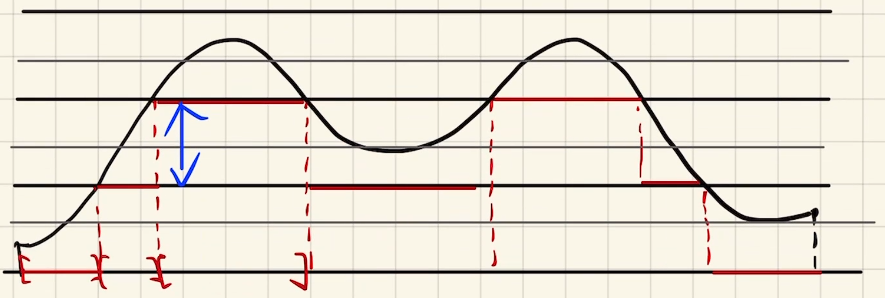
\includegraphics[width=0.55\textwidth]{figure/2.2-1} %图片的名称或者路径之中有空格会出问题 
						\caption{对$f$ 值域进行分划} % 图片标题
						\label{pic 2.1}
					\end{figure}
				
					\newpage
					\item[$2^{\circ}$]$f$ is unbounded. (\underline{idea}: truncation,将$f$ 截断为一列有界函数列,并逐点收敛于$f$)\\
					Let
					\begin{align}
						f_{k}(x) = 
						\begin{cases}
							f(x) , \,\, &if \,\, f(x) \leq k \\
							k , &if \,\, f(x) > k
						\end{cases}
					\end{align}	
					Then $f_{k}(x) \to f(x)$, $\forall x \in \R^d$. \\
					Since $f_k$ is bounded, by the previous result in $1^{\circ}$, \\
					For each $k$, $\exists$ a sequence of simple functions $\{ \psi_{kn} \}_{n = 1}^{\infty}$, $\st$
					\begin{align}
						\psi_{kn}(x) \to f_{k}(x) , \,\, \forall x
					\end{align}
					So we get
					\begin{align}
						\begin{matrix}
							&\textcolor{red}{\psi_{11}} \,\, &\psi_{12} \,\, &\psi_{13} \,\, &\cdots \,\, &\to \,\, &f_1 \\
							&\psi_{21} \,\, &\textcolor{red}{\psi_{22}} \,\, &\psi_{23} \,\, &\cdots \,\, &\to \,\, &f_2 \\
							&\psi_{31} \,\, &\psi_{32} \,\, &\textcolor{red}{\psi_{33}} \,\, &\cdots \,\, &\to \,\, &f_3 \\
							&\cdots \,\, &\cdots \,\, &\cdots \,\, &\cdots \,\, &\cdots \,\, &\cdots \\
							&\cdots \,\, &\cdots \,\, &\cdots \,\, &\cdots \,\, &\cdots \,\, &\downarrow \\
							& & & & & &\textcolor{red}{f} \\
						\end{matrix}
					\end{align}
					From the previous results in $1^{\circ}$, we get
					\begin{align}
						\left| \psi_{kn}(x) - f_k(x) \right| \leq \frac{1}{2^n}
					\end{align}
					Let $n = k$, then $\left| \psi_{kk}(x) - f_k(x) \right| \leq \frac{1}{2^k}$. Let $\varphi_k = \psi_{kk}$, then
					\begin{align}
						\left| \varphi_{k}(x) - f(x) \right| 
						\leq \left| \varphi_{k}(x) - f_{k}(x) \right| + \left| f_{k}(x) - f(x) \right|
					\end{align}
					Since $f_{k}(x) \to f(x)$, we get $\varphi_{k}(x) \to f(x)$, $\forall x$, where $\{ \varphi_k = \psi_{kk} \}_{k = 1}^{\infty}$ are simple functions.
				\end{enumerate}
				
				\item[(2)]变号函数$f : \R^d \longrightarrow [-\infty , \infty]$.\\
				We denote that
				\begin{align}
					f^{+}(x) &\coloneqq \max{\{ f(x) , 0 \}} \\
					f^{-}(x) &\coloneqq \max{\{ -f(x) , 0 \}}
				\end{align}
				By the previous results in (1), there exist sequences of simple functions $\{ \varphi_k \}_{k = 1}^{\infty} , \{ \psi_k \}_{k = 1}^{\infty}$, $\st$
				\begin{align}
					\varphi_k \to f^{+} \,\, and \,\, \psi_{k} \to f^{-} \,\, pointwisely
				\end{align}
				We can observe that $f = f^+ - f^-$ and $\left| f \right| = f^+ - f^-$.\\
				Let $\phi_{k}(x) = \varphi_{k}(x) - \psi_{k}(x)$, then $\phi_k$ is a simple function with $\phi_k \to f$ pointwisely.
			\end{enumerate}
		\end{proof}
	\end{thm}

\newpage
\paragraph{阶梯函数逼近可测函数}
	在证明了可测函数可由简单函数逼近后,我们更进一步,来说明可测函数可由更加简单的\textbf{阶梯函数}来逼近.
	
	\vspace{2em}
	先给出\textbf{阶梯函数}的定义.
	\begin{defn}\label{def 2.2.3}
		A \underline{\textcolor{blue}{\textbf{step function}}} is a finite sum
		\begin{align}
			f = \sum_{k = 1}^{N}{a_{k} \chi_{R_k}} , \,\, where \,\, R_k \,\, is \,\, a \,\, rectangle
		\end{align}
	
		\begin{rmk}
			阶梯函数$\&$ 简单函数的区别在于,简单函数是作用于有限个\textbf{可测集$E_k$},而阶梯函数是作用于有限个\textbf{矩形$R_k$}.
		\end{rmk}
	\end{defn}

	\vspace{2em}
	下面的定理说明了measurable functions are almost step functions.
	\begin{thm}\label{thm 2.2.2}
		Suppose $f$ is measurable on $\R^d$. Then there exists a sequence of step functions $\{ \psi_k \}_{k = 1}^{\infty}$, $\st$
		\begin{align}
			\lim_{k \to \infty}{\psi_{k}(x)} = f(x) , \,\, a.e. \,\, x
		\end{align}
	
		\begin{rmk}
			首先介绍函数列收敛点集的几种不同的等价表述:
			\begin{align}
				&\{ x \mid \forall \epsilon > 0 , \exists N \in \N , \forall n \geq N , \,\, \left| f_{n}(x) - f(x) \right| < \epsilon \} \\
				\Leftrightarrow 
				&\{ x \mid \forall n \in \N , \exists N \in \N , \forall k \geq N , \,\, \left| f_{k}(x) - f(x) \right| < \frac{1}{n} \} \\
				\Leftrightarrow 
				&\bigcap_{n = 1}^{\infty} \bigcup_{N = 1}^{\infty} \bigcap_{k = N}^{\infty} \{ x \mid \,\, \left| f_{k}(x) - f(x) \right| < \frac{1}{n} \}
			\end{align}
			从而可以得到函数列发散点集(Negation):
			\begin{align}
				&\{ x \mid \exists n \in \N , \forall N \in \N , \exists k \geq N , \,\, \left| f_{k}(x) - f(x) \right| \geq \frac{1}{n} \} \\
				\Leftrightarrow 
				&\bigcup_{n = 1}^{\infty} \bigcap_{N = 1}^{\infty} \bigcup_{k = N}^{\infty} \{ x \mid \,\, \left| f_{k}(x) - f(x) \right| \geq \frac{1}{n} \} \\
				\Leftrightarrow
				&\textcolor{red}{\bigcap_{N = 1}^{\infty} \bigcup_{k = N}^{\infty} \{ x \mid \,\, f_{k}(x) \neq f(x) \}}
			\end{align}
		\end{rmk}
	
		\vspace{2em}
		\begin{proof}
			(证明思路:先用阶梯函数逼近简单函数,再用简单函数逼近可测函数.)
			\begin{center}
				It suffices to show that $\chi_E$ can be approxiamted by step functions, for any measurable set $E$.
			\end{center}
			According to Thm\ref{thm 1.3.4} (\rmnum{4}) \\
			Let $f = \chi_E$, then $\forall \epsilon > 0$, $\exists$ cubes $\overset{N}{\underset{j = 1}{\bigcup}}{Q_j}$, $\st$
			\begin{align}
				m(E \,\, \triangle \,\, \bigcup_{j = 1}^{N}{Q_j}) \leq \epsilon
			\end{align}
			By considering the grid formed by extending the sides of these cubes, there exists almost disjoint rectangles $\{ \widetilde{R}_j \}_{j = 1}^{M}$, $\st$
			\begin{align}
				\bigcup_{j = 1}^{N}{Q_j} = \bigcup_{j = 1}^{M}{\widetilde{R}_j}
			\end{align}
			By taking ranctangles $R_j$ contained in $\widetilde{R}_j$, we can find a collection of disjoint rectangles $\{ R_j \}_{j = 1}^{M}$, $\st$
			\begin{align}
				m(E \,\, \triangle \,\, \bigsqcup_{j = 1}^{M}{R_j}) \leq 2\epsilon
			\end{align}
			For every $k \in \N$, there exists disjoint rectangles $\{ R_j \}_{j = 1}^{M}$, $\st$
			\begin{align}
				m(E \,\, \triangle \,\, \bigsqcup_{j = 1}^{M}{R_j}) \leq \frac{1}{2^{k + 1}}
			\end{align}
			There also exists a step function $\psi_k$
			\begin{align}
				\psi_{k}(x) \coloneqq \chi_{\bigcup_{j = 1}^{M}{R_j}}(x) = \sum_{j = 1}^{M}{\chi_{R_j}(x)}
			\end{align}
			Let
			\begin{align}
				E_k \coloneqq \{ x \mid f_{k}(x) \neq f(x) \}
			\end{align}
			Since $E_k \subset E \,\, \triangle \,\, \overset{M}{\underset{j = 1}{\bigsqcup}}{R_j}$, then $m(E_k) \leq \frac{1}{2^k}$. Let\footnote{根据\textcolor{red}{\textbf{注}}中式(2.56),$F$ 即为函数列$\{ \psi_k \}_{k = 1}^{\infty}$ 的发散点集,从而$\psi_{k}(x) \to f(x)$ 在$F^c$ 上收敛.}
			\begin{align}
				F_j = \bigcup_{j = k + 1}^{\infty}{E_j} , \,\, F = \bigcap_{k = 1}^{\infty}{F_k}
			\end{align}
			Then $\psi_{k}(x) \to f(x)$, $\forall x \in F^c$. Since
			\begin{align}
				m(F) &\leq m(F_k) , \,\, \forall k \in \N \\
				m(F_k) &= m(\bigcup_{j = k + 1}^{\infty}{E_j}) \leq \sum_{j = k + 1}^{\infty}{m(E_j)} \leq \frac{1}{2^k}
			\end{align}
			Therefore, $m(F) = 0$. $\underset{k \to \infty}{\lim}{\psi_{k}(x)} = f(x)$, $a.e.$ $x$.
		\end{proof}
	\end{thm}

\chapter{$Integration \,\, Theory$}
\section{$The \,\, Lebesgue \,\, integral$}
	$Lebesgue$ $Integral$ 的构造可以分为三步,分别为构造下列函数的积分:
	\begin{enumerate}
		\item \textbf{Simple functions} 
	
		\item \textbf{Non-negative measurable functions}
		\begin{align}
			\int f \coloneqq \sup{\{ \int \varphi \mid \varphi \,\, simple , \,\, 0 \leq \varphi \leq f \}}
		\end{align}
	
		\item \textbf{General case}
		\begin{align}
			f &= f^{+} - f^{-} \\
			\int f &\coloneqq \int f^{+} - \int f^{-}
		\end{align}
	\end{enumerate}

\subsection{$Simple \,\, functions$}
\paragraph{定义}
	下面先给出非负简单函数在\textbf{标准形式}下的\textbf{积分}定义.
	\begin{defn}\label{def 3.1.1}
		If $\varphi$ is a non-negative simple function with \textbf{standard representation}
		\begin{align}
			\varphi(x) = \sum_{k = 1}^{M}{a_k \chi_{E_k}(x)}
		\end{align}
		We define the \underline{\textcolor{blue}{\textbf{Lebesgue integral}}} of $\varphi$ by
		\begin{align}
			\int_{\R^d}{\varphi(x) dx} = \sum_{k = 1}^{M}{a_k m(E_k)}
		\end{align}
		If $E$ is a measurable subset of $\R^d$ with finite measure, then
		\begin{align}
			\varphi(x) \chi_{E}(x) = \sum_{k = 1}^{M}{a_k \chi_{E_k}(x) \chi_{E}(x)} = \sum_{k = 1}^{M}{a_k \chi_{E_k \cap E}(x)}
		\end{align}
		is also a simple function, and define
		\begin{align}
			\int_{E}{\varphi(x) dx} = \int_{\R^d}{\varphi(x) \chi_{E}(x) dx}
		\end{align}
		
		\newpage
		\begin{rmk}
			\begin{itemize}
				\item 此处仅对\textbf{标准形式}定义了积分. 事实上,此处定义的积分与简单函数的表达形式无关(即\textcolor{red}{\textbf{Property 1.}}).
				
				\item 关于记号,当测度非常明确时,大多数情况下可简写,如
				\begin{align}
					\int_{E}{\varphi(x) dx} \,\, &\Rightarrow \,\, \int_{E}{\varphi} \\
					\int_{\R^d}{\varphi(x) dx} &\Rightarrow \,\, \int{\varphi}
				\end{align}
				当为了强调我们选择了何种测度$\mu$ 时,还可用以下的记号:
				\begin{align}
					\int_{E}{\varphi(x) d\mu(x)}
				\end{align}
			\end{itemize}
		\end{rmk}
	\end{defn}

\vspace{2em}
\paragraph{Property}
	下面给出简单函数积分的性质.
	
	\begin{enumerate}
		\item[\textcolor{red}{\textbf{Property 1.}}]\textbf{Independence of the representation}.\\
		If $\varphi = \overset{N}{\underset{k = 1}{\sum}}{a_k \chi_{E_k}}$ is any representation of $\varphi$, then
		\begin{align}
			\int \varphi = \sum_{k = 1}^{N}{a_k m(E_k)}
		\end{align}
		
		\vspace{2em}
		在证明这个性质之前,先来证明一条引理.(书\footnote{参考书籍:\textbf{《$Real \,\, Analysis -- Measure \,\, Theroy, \,\, Integration, \,\, \& \,\, Hilbert \,\, Spaces$》--- $Elias \,\, M. \,\, Stein$}}Exercises Of Chapter 2 的第1题)
		
		\begin{lemma}\label{lemma 3.1.1}
			Given a collection of sets $\{ F_k \}_{k = 1}^{n}$, there exists another collection $\{ \widetilde{F}_j \}_{j = 1}^{N}$ \\
			with $N = 2^n - 1$, so that
			\begin{align}
				(\rmnum{1})&. \hspace*{2em} \bigcup_{k = 1}^{n}{F_k} = \bigcup_{j = 1}^{N}{\widetilde{F}_j} \\
				(\rmnum{2})&. \hspace*{2em} \{ \widetilde{F}_j \}_{j = 1}^{N} \,\, are \,\, disjoint \\
				(\rmnum{3})&. \hspace*{2em} F_k = \bigcup_{\widetilde{F}_j \subset F_k}{\widetilde{F}_j}
			\end{align}
		
			\vspace{2em}
			\begin{proof}
				Consider the collection
				\begin{align}
					\mathcal{F} \coloneqq \{ \bigcup_{k = 1}^{n}{G_k} - \bigcap_{k = 1}^{n}{F_{k}^{c}} \,\, \Big| \,\, G_k \,\, denotes \,\, F_k \,\, or \,\, F_{k}^c \}
				\end{align}
			\end{proof}
		\end{lemma}
	
		\newpage	
		下面来证明原命题.
		\begin{proof}
			 According to Lemma \ref{lemma 3.1.1}, there exists another decompositon of $\overset{N}{\underset{k = 1}{\bigcup}}{E_k}$, i.e.
			 \begin{align}
			 	\bigcup_{j = 1}^{M}{\widetilde{E}_j} = \bigcup_{k = 1}^{N}{E_k}
			 \end{align}
		 	where $\{ \widetilde{E}_j \}_{j = 1}^M$ are disjoint, and for each $1 \leq k \leq M$,
		 	\begin{align}
		 		E_k = \bigcup_{\widetilde{E}_j \subset E_k}{\widetilde{E}_j}
		 	\end{align}
	 		Let
	 		\begin{align}
	 			\widetilde{a}_j \coloneqq \sum_{\widetilde{E}_j \subset E_k}{a_k}
	 		\end{align}
 			Then clearly
 			\begin{align}
 				\varphi = \sum_{j = 1}^{M}{\widetilde{a}_j \chi_{\widetilde{E}_j}}
 			\end{align}
 			Since $\{ \widetilde{E}_j \}_{j = 1}^M$ are disjoint, we get
 			\begin{align}
 				\int{\varphi} = \sum_{j = 1}^{M}{\widetilde{a}_j m(\widetilde{E}_j)} = \sum_{j = 1}^{M}{\sum_{\widetilde{E}_j \subset E_k}{a_k m(\widetilde{E}_j)}} = \sum_{k = 1}^{N}{a_k m(E_k)}
 			\end{align}
		\end{proof}
		
		\vspace{2em}
		\item[\textcolor{red}{\textbf{Property 2.}}]\textbf{Linearity}.\\
		If $\varphi$ and $\psi$ are non-negative simple, and $a , b \geq 0$, then
		\begin{align}
			\int{(a \varphi + b \psi)} = a\int{\varphi} + b\int{\psi}
		\end{align}
		
		\vspace{2em}
		\begin{proof}
			下面分为两步来证明.
			\begin{enumerate}
				\item[(a)]$\forall c \geq 0$, $\int{c \varphi} = c \int{\varphi}$.\\
				Suppose $\varphi = \overset{M}{\underset{k = 1}{\sum}}{a_k \chi_{E_k}}$, where $\{ E_k \}_{k = 1}^{M}$ are disjoint. Then
				\begin{align}
					c\varphi = \sum_{k = 1}^{M}{c a_k \chi_{E_j}}
				\end{align}
				is also a non-negative simple function. Therefore,
				\begin{align}
					\int{c\varphi} = \sum_{k = 1}^{M}{c a_k m(E_k)} = c\sum_{k = 1}^{M}{a_k m(E_k)} = c\int{\varphi}
				\end{align}
			
				\item[(b)]$\int{(\varphi + \psi)} = \int{\varphi} + \int{\psi}$.\\
				Suppose
				\begin{align}
					\varphi = \sum_{k = 1}^{M}{a_k \chi_{E_k}} , \,\, \psi = \sum_{j = 1}^{N}{b_j \chi_{F_j}}
				\end{align}
				where both $\{ E_k \}_{k = 1}^{M}$ and $\{ F_j \}_{j = 1}^{N}$ are disjoint and $\R^d = \overset{M}{\underset{k = 1}{\bigcup}}{E_k} = \overset{N}{\underset{j = 1}{\bigcup}}{F_j}$. Since
				\begin{align}
					E_k = E_k \cap \R^d = E_k \cap \bigsqcup_{j = 1}^{N}{F_j} = \bigsqcup_{j = 1}^{N}{(E_k \cap F_j)}
				\end{align}
				Then
				\begin{align}
					\varphi = \sum_{k = 1}^{M}{a_k \chi_{E_k}} = \sum_{k = 1}^{M}{a_k \chi_{\bigsqcup_{j = 1}^{N}{(E_k \cap F_j)}}} = \sum_{k = 1}^{M}{\sum_{j = 1}^{N}{a_k \chi_{E_k \cap F_j}}}
				\end{align}
				Similarly
				\begin{align}
					\psi = \sum_{j = 1}^{N}{b_j \chi_{F_j}} = \sum_{j = 1}^{N}{b_k \chi_{\bigsqcup_{k = 1}^{M}{(E_k \cap F_j)}}} = \sum_{j = 1}^{N}{\sum_{k = 1}^{M}{b_k \chi_{E_k \cap F_j}}}
				\end{align}
				Therefore
				\begin{align}
					\varphi + \psi &= \sum_{j , k}{(a_k + b_j)\chi_{E_k \cap F_j}} \\
					\int{(\varphi + \psi)} &= \sum_{j , k}{(a_k + b_j)m(E_k \cap F_j)} \\
					&= \sum_{j , k}{a_k m(E_k \cap F_j)} + \sum_{j , k}{b_j m(E_k \cap F_j)} \\
					&= \int{\varphi} + \int{\psi}
				\end{align}
			\end{enumerate}
		\end{proof}
		
		\vspace{2em}
		\item[\textcolor{red}{\textbf{Property 3.}}]\textbf{Monotonicity}.\\
		If $\varphi \leq \psi$ are non-negative and simple, then
		\begin{align}
			\int{\varphi} \leq \int{\psi}
		\end{align}
	
		\vspace{2em}
		\begin{proof}
			Suppose
			\begin{align}
				\varphi = \sum_{k = 1}^{M}{a_k \chi_{E_k}} , \,\, \psi = \sum_{j = 1}^{N}{b_j \chi_{F_j}}
			\end{align}
			where both $\{ E_k \}_{k = 1}^{M}$ and $\{ F_j \}_{j = 1}^{N}$ are disjoint. Similar to the proof in Property 2, we get
			\begin{align}
				\psi - \varphi = \sum_{j , k}{(b_j - a_k) \chi_{E_k \cap F_j}}
			\end{align}
			Since $\varphi(x) \leq \psi(x)$, $\forall x \in \R^d$, then $\psi - \varphi$ is non-negative and simple. Therefore,
			\begin{align}
				\int{(\psi - \varphi)} = \sum_{j , k}{(b_j - a_k) m(E_k \cap F_j)} \geq 0 \,\, \Rightarrow \,\, \int{\varphi} \leq \int{\psi}
			\end{align}
		\end{proof}
	
		\vspace{2em}
		\item[\textcolor{red}{\textbf{Property 4.}}]\textbf{Additivity}.\\
		If $\{ E_k \}_{k = 1}^{\infty}$ are disjoint subsets of $\R^d$ with finite measure, then
		\begin{align}
			\int_{\bigcup_{k = 1}^{\infty}{E_k}}{\varphi} = \sum_{k = 1}^{\infty}{\int_{E_k}{\varphi}}
		\end{align}
		
		\vspace{2em}
		\begin{rmk}
			首先回顾$abstract$ $measure$ 的定义.
			\begin{defn}\label{def 3.1.2}
				Let $X$ be a set and let $\mathcal{M}$ be a $\sigma-algebra$ on $X$.\\
				A \underline{\textcolor{blue}{\textbf{measure}}} on $\mathcal{M}$ is a function $\mu : \mathcal{M} \longrightarrow [0 , \infty]$, $\st$
				\begin{enumerate}
					\item[(\rmnum{1})]$\mu(\varnothing) = 0$.
					
					\item[(\rmnum{2})]If $\{ E_j \}_{j = 1}^{\infty} \subset \mathcal{M}$ are disjoint, then
					\begin{align}
						\mu(\bigcup_{j = 1}^{\infty}{E_j}) = \sum_{j = 1}^{\infty}{\mu(E_j)}
					\end{align}
				\end{enumerate}
			\end{defn}
			
			\vspace{2em}
			回到我们积分的性质上来. 下面我们将说明,对于任一给定的非负简单函数$\varphi$,将$\varphi$ 在任一可测集$A$ 上的积分看作$Lebesgue \,\, \sigma-algebra \,\, \mathcal{L}$ 上的映射,则该映射为定义在$\mathcal{L}$ 上的测度.(从而Property 4.作为测度的必要条件自然成立)
			
			\vspace{2em}
			\begin{proposition}\label{prop 3.1.1}
				For any fixed non-negative and simple function $\varphi$, the map
				\begin{align}
					\mu : \mathcal{L} &\longrightarrow [0 , \infty] \\
					A &\longmapsto \int_{A}{\varphi}
				\end{align}
				is a measure on $\mathcal{L}$.
				
				\newpage
				\begin{proof}
					Suppose $\{ A_j \}_{j = 1}^{\infty} \subset \mathcal{L}$ are disjoint, and
					\begin{align}
						\varphi = \sum_{k = 1}^{M}{a_k \chi_{E_k}} , \,\, where \,\, \{ E_k \}_{k = 1}^{M} \,\, are \,\, disjoint
					\end{align}
					Let $A = \overset{\infty}{\underset{j = 1}{\bigcup}}{A_j}$, then
					\begin{align}
						\int_{\bigcup_{j = 1}^{\infty}{A_j}}{\varphi} 
						= \int_{A}{\varphi} 
						= \int{\varphi \chi_A} 
						&= \int{(\sum_{k = 1}^{M}{a_k \chi_{E_k \cap A}})} \\
						&= \sum_{k = 1}^{M}{a_k m(E_k \cap A)} \\
						&= \sum_{k = 1}^{M}{a_k m(E_k \cap (\bigcup_{j = 1}^{\infty}{A_j}))} \\
						&= \sum_{k = 1}^{M}{a_k m(\bigsqcup_{j = 1}^{\infty}{(E_k \cap A_j)})} \\
						&= \sum_{k = 1}^{M}{a_k \sum_{j = 1}^{\infty}{m(E_k \cap A_j)}} \\
						&= \sum_{k = 1}^{M}{\sum_{j = 1}^{\infty}{a_k m(E_k \cap A_j)}}
					\end{align}
					Since positive series always converges in $[0 , \infty]$, then
					\begin{align}
						\int_{A}{\varphi} 
						= \sum_{k = 1}^{M}{\sum_{j = 1}^{\infty}{a_k m(E_k \cap A_j)}} 
						= \sum_{j = 1}^{\infty}{\sum_{k = 1}^{M}{a_k m(E_k \cap A_j)}} 
						= \sum_{j = 1}^{\infty}{\int_{A_j}{\varphi}}
					\end{align}
					Therefore, \uwave{\textbf{the integral on any non-negative simple function is accually a measure on $\mathcal{L}$}}.
				\end{proof}
			\end{proposition}
		\end{rmk}
	\end{enumerate}

\newpage
\subsection{$Non-negative \,\, measurable \,\, functions$}
	为了讨论的方便,先给出\textbf{非负可测函数}的一个记号.
	\begin{align}
		\mathcal{M}^{+} \coloneqq \{ all \,\, non-negative \,\, measurable \,\, functions \}
	\end{align}

\vspace{2em}
\paragraph{定义}
	下面给出非负可测函数的积分的定义.
	\begin{defn}\label{def 3.1.3}
		For $f \in \mathcal{M}^{+}$, we define
		\begin{align}
			\int{f(x) dx} \coloneqq \sup{\{ \int{\varphi(x) dx} \mid 0 \leq \varphi \leq f , \,\, \varphi \,\, simple \}}
		\end{align}
		
		\begin{rmk}
			此处对Non-negative measurable function 积分的定义兼容定义 \ref{def 3.1.1} 中对Non-negative simple function 积分的定义,具体表现为:$\forall \varphi_0$ non-negative and simple,
			\begin{align}
				\sup{\{ \int{\varphi(x) dx} \mid 0 \leq \varphi \leq \varphi_0 , \,\, \varphi \,\, simple \}} = \int{\varphi_0 (x) dx}
			\end{align}
		\end{rmk}
	\end{defn}

\vspace{2em}
\paragraph{性质}
	下面来验证定义 \ref{def 3.1.3} 中定义的积分满足几条基本性质.
	\begin{enumerate}
		\item[\textcolor{red}{\textbf{Property 1.}}]\textbf{Monotonicity}.\\
		Let $f , g \in \mathcal{M}^{+}$. Then
		\begin{align}
			\int{f} \leq \int{g} \,\,\,\, if \,\,\,\, f \leq g
		\end{align}
		
		\vspace{2em}
		\begin{proof}
			Let
			\begin{align}
				A &= \{ \varphi \,\, simple \mid 0 \leq \varphi \leq f \} \\
				B &= \{ \psi \,\, simple \mid 0 \leq \psi \leq g \}
			\end{align}
			Then for all $\varphi \in A$, $0 \leq \varphi \leq f \leq g$ $\Rightarrow$ $\varphi \in B$ $\Rightarrow$ $A \subset B$. Since
			\begin{align}
				\int{f} = \sup_{\varphi \in A}{\{ \int{\varphi} \}} , \,\, \int{g} = \sup_{\psi \in B}{\{ \int{\psi} \}}
			\end{align}
			Therefore
			\begin{align}
				\int{f} \leq \int{g}
			\end{align}
		\end{proof}
	
		\newpage
		
		\item[\textcolor{red}{\textbf{Property 2.}}]\textbf{齐次性}.\\
		Let $f \in \mathcal{M}^{+}$. If $c \geq 0$, then
		\begin{align}
			\int{cf} = c\int{f}
		\end{align}
	
		\vspace{2em}
		\begin{proof}
			Assume $c > 0$. Then
			\begin{align}
				\int{cf} 
				&= \sup{\{ \int{\varphi} \mid 0 \leq \varphi \leq cf , \,\, \varphi \,\, simple \}} \\
				&= \sup{\{ \int{\varphi} \mid 0 \leq \frac{\varphi}{c} \leq f , \,\, \varphi \,\, simple \}} \\
				&\overset{\psi \, = \, \frac{\varphi}{c}}{=} \sup{\{ \int{c\psi} \mid 0 \leq \psi \leq f , \,\, \psi \,\, simple \}} \\
				&= c \sup{\{ \int{\psi} \mid 0 \leq \psi \leq f , \,\, \psi \,\, simple \}} \\
				&= c \int{f}
			\end{align}
		\end{proof}
	\end{enumerate}

\paragraph{单调收敛定理}
	下面我们正式迈入实分析的\textbf{“大门”},介绍第一个\textbf{收敛定理}.
	\begin{thm}\label{thm 3.1.2}
		\textbf{The Monotone Convergence Theorem}.\\
		If $\{ f_n \}_{n = 1}^{\infty} \subset \mathcal{M}^{+}$, $f_j \leq f_{j + 1}$ for all $j$, and $\underset{n \to \infty}{\lim}{f_n} = f$, then
		\begin{align}
			\int{f} = \lim_{n \to \infty}{\int{f_n}}
		\end{align}
		
		\vspace{1em}
		\begin{rmk}
			\begin{itemize}
				\item 此即为\textbf{“单调收敛定理”},这个定理说明了对于\textbf{单调递增}的\textbf{非负可测}函数列,\\
				其\uwave{\textcolor{red}{\textbf{积分与极限可交换次序}}}. 具体表现为
				\begin{align}
					\int{f} = \int{\lim_{n \to \infty}{f_n}} = \lim_{n \to \infty}{\int{f_n}}
				\end{align}
				
				\vspace{2em}
				\item 该定理还说明了,我们可以给出非负可测函数的另一个更自然的等价定义,即用非负简单函数列的积分逼近非负可测函数的积分.
				\begin{defn}\label{def 3.1.4}
					For $f \in \mathcal{M}^{+}$, we can also define
					\begin{align}
						\int{f} \coloneqq \lim_{n \to \infty}{\int{\varphi_n}}
					\end{align}
					where $\varphi_n \to f$ and $0 \leq \varphi_1 \leq \varphi_2 \leq \cdots \leq f$ by Thm \ref{thm 2.2.1}.
				\end{defn}
				并且该定理说明了该积分定义的\textbf{唯一性}及\textbf{well-defined}.
			\end{itemize}
		\end{rmk}
	
		\newpage
		在证明定理前,先来证明一个引理(将定理 \ref{thm 1.3.3} (\rmnum{1}) 拓展到一般的抽象测度上).
		\begin{lemma}\label{lemma 3.1.3}
			Let $X$ be a set, $\mathcal{M}$ be a $\sigma-algebra$ on $X$, $\mu : \mathcal{M} \longrightarrow [0 , \infty]$ be a measure on $\mathcal{M}$.\\
			If $\{ E_n \}_{n = 1}^{\infty} \subset \mathcal{M}$, $E_n \nearrow E$, then
			\begin{align}
				\lim_{n \to \infty}{\mu(E_n)} = \mu(E)
			\end{align}
		
			\vspace{2em}
			\begin{proof}
				证明过程与Thm \ref{thm 1.3.3} 完全一致(仅用到了测度的可数可加性).\\
				Let $S_1 = E_1$, $S_k = E_k - E_{k - 1}$, $\forall k \geq 2$. Then $\{ S_k \}_{n = 1}^{\infty} \subset \mathcal{M}$ are disjoint.\\
				Since $E = \overset{\infty}{\underset{k = 1}{\bigcup}}{E_k} = \overset{\infty}{\underset{k = 1}{\bigcup}}{S_k}$, then
				\begin{align}
					\mu(E) 
					= \mu(\bigsqcup_{k = 1}^{\infty}{S_k}) 
					= \sum_{k = 1}^{\infty}{\mu(S_k)} 
					= \lim_{n \to \infty}{\sum_{k = 1}^{n}{\mu(S_k)}} 
					= \lim_{n \to \infty}{\mu(\bigsqcup_{k = 1}^{n}{S_k})} 
					= \lim_{n \to \infty}{\mu(E_n)}
				\end{align}
			\end{proof}
		\end{lemma}
		
		\vspace{2em}
		下面证明原定理.
		\begin{proof}
			\begin{itemize}
				\item $\underset{n \to \infty}{\lim}{\int{f_n}} \leq \int{f}$.\\
				Since $f_n \leq f$, $\forall n$, then
				\begin{align}
					\int{f_n} \leq \int{f} , \,\, \forall n
				\end{align}
				Since $\{ \int{f_n} \}_{n = 1}^{\infty}$ always converges in $[0 , \infty]$, then let $n \to \infty$, we get
				\begin{align}
					\lim_{n \to \infty}{\int{f_n}} \leq \int{f}
				\end{align}
				
				\vspace{2em}
				\item $\underset{n \to \infty}{\lim}{\int{f_n}} \geq \int{f}$.\\
				Fix $0 < \alpha < 1$, for any $0 \leq \varphi \leq f$ simple, let
				\begin{align}
					E_n = \{ x \mid f_{n}(x) \geq \alpha \varphi(x) \}
				\end{align}
				Then since $\forall x \in E_n$, we have $f_{n + 1}(x) \geq f_{n}(x) \geq \alpha \varphi(x)$ $\Rightarrow$ $x \in E_{n + 1}$ $\Rightarrow$ $E_n \subset E_{n + 1}$.\\
				Then $E_n \nearrow$. Since
				\begin{align}
					\int_{\R^d}{f_n} \geq \int_{E_n}{f_n} \geq \int_{E_n}{\alpha \varphi} ,  \,\, \forall n
				\end{align}
				Let $n \to \infty$, we get
				\begin{align}
					\lim_{n \to \infty}{\int_{\R^d}{f_n}} \geq \lim_{n \to \infty}{\int_{E_n}{\alpha \varphi}}
				\end{align}
				\newpage
				Then we have to calculate \textcolor{red}{$\underset{n \to \infty}{\lim}{\int_{E_n}{\alpha \varphi}}$}:
				
				\vspace{2em}
				\begin{itemize}
					\item Since $\alpha \varphi$ is non-negative and simple, by Prop \ref{prop 3.1.1}, the map
					\begin{align}
						\mu : \mathcal{L} &\longrightarrow [0 , \infty] \\
						E &\longmapsto \int_{E}{\alpha \varphi}
					\end{align}
					is a measure on the collection of Lebesgue measurable sets $\mathcal{L}$. (\textcolor{red}{\textbf{将积分视作测度}}) \\
					Since $\{ E_n \}_{n = 1}^{\infty} \subset \mathcal{L}$ and $E_n \nearrow$, by Lemma \ref{lemma 3.1.3}, we get
					\begin{align}
						\lim_{n \to \infty}{\mu(E_n)} = \mu(\bigcup_{n = 1}^{\infty}{E_n})
					\end{align}
					i.e.
					\begin{align}
						\lim_{n \to \infty}{\int_{E_n}{\alpha \varphi}} = \int_{\bigcup_{n = 1}^{\infty}{E_n}}{\alpha \varphi}
					\end{align}
					For all $x \in \R^d$, since $\alpha \varphi(x) < f(x)$ and $f_n \to f$, there exists $N_x \in \N$, $\st$
					\begin{align}
						f_{n}(x) \geq \alpha \varphi(x) , \,\, \forall n \geq N_x
					\end{align}
					which indicates $x \in E_{N_x}$ for some $N_x$. Therefore
					\begin{align}
						\bigcup_{n = 1}^{\infty}{E_n} = \R^d \,\, \Rightarrow \,\, 
						\textcolor{red}{\lim_{n \to \infty}{\int_{E_n}{\alpha \varphi}}} 
						= \int_{\bigcup_{n = 1}^{\infty}{E_n}}{\alpha \varphi} 
						= \textcolor{red}{\int_{\R^d}{\alpha \varphi}}
					\end{align}
				\end{itemize}
			
				\vspace{2em}
				Therefore, we get
				\begin{align}
					\lim_{n \to \infty}{\int_{\R^d}{f_n}} 
					\geq \lim_{n \to \infty}{\int_{E_n}{\alpha \varphi}} 
					= \int_{\R^d}{\alpha \varphi}
				\end{align}
				Let $\alpha \to 1$, then
				\begin{align}
					\lim_{n \to \infty}{\int_{\R^d}{f_n}} 
					\geq \int_{\R^d}{\varphi}
				\end{align}
				Since $\varphi$ is arbitratry, taking the supremum over $\varphi$, we get
				\begin{align}
					\lim_{n \to \infty}{\int_{\R^d}{f_n}} 
					\geq \sup{\{ \int_{\R^d}{\varphi} \mid 0 \leq \varphi \leq f , \,\, \varphi \,\, simple \}}
					= \int{f}
				\end{align}
			\end{itemize}
		\end{proof}
	\end{thm}

\newpage
\paragraph{函数项级数的可数可加性}
	接下来我们将给出\textbf{单调收敛定理}在\textbf{函数项级数}上的表达形式,它说明了对于\textbf{非负可测函数项级数},其\uwave{\textbf{积分与求和可交换次序}}.
	
	\vspace{2em}
	在此之前,先来证明有限项的情况.
	\begin{center}
		(此也可视作非负可测函数积分的\textcolor{red}{\textbf{Property}} \textbf{线性性}的一部分.)
	\end{center}
	\begin{proposition}\label{prop 3.1.2}
		\textbf{Linearity}.\\
		If $f , g \in \mathcal{M}^{+}$, then
		\begin{align}
			\int{(f + g)} = \int{f} + \int{g}
		\end{align}
	
		\vspace{2em}
		\begin{proof}
			By Thm \ref{thm 2.2.1} and Thm \ref{thm 3.1.2}, there exists sequences of non-negative and simple functions $\{ \varphi_n \}_{n = 1}^{\infty}$ and $\{ \psi_n \}_{n = 1}^{\infty}$, $\varphi_n \to f$ and $\psi_n \to g$, $\st$
			\begin{align}
				\int{f} = \lim_{n \to \infty}{\int{\varphi_n}} , \,\, \int{g} = \lim_{n \to \infty}{\int{\psi_n}}
			\end{align}
			Since $\varphi_n + \psi_n$ is still non-negative and simple, then \\
			By the Linearity of integral on non-negative and simple functions, (\textcolor{red}{\textbf{Property 2.}} in $\S 3.1.1$)
			\begin{align}
				\int{(\varphi_n + \psi_n)} = \int{\varphi_n} + \int{\psi_n}
			\end{align}
			Let $n \to \infty$, by Thm \ref{thm 3.1.2}, we get (\textbf{极限与积分交换次序})
			\begin{align}
				\int{(f + g)} = \int{f} + \int{g}
			\end{align}
		\end{proof}
	\end{proposition}
	
	根据Prop \ref{prop 3.1.2},由归纳法,容易得到其对任意\textbf{有限项}函数项级数都成立.
	
	\newpage
	下面给出\textbf{函数项级数}上的\textbf{单调收敛定理}.
	\begin{thm}\label{thm 3.1.4}
		\textbf{Monotone Convergence Theorem (MCT , series version)}.\\
		If $\{ f_n \}_{n = 1}^{\infty} \subset \mathcal{M}^{+}$ and $f = \overset{\infty}{\underset{n = 1}{\sum}}{f_n}$, then
		\begin{align}
			\int{f} = \sum_{n = 1}^{\infty}{\int{f_n}}
		\end{align}
	
		\vspace{1em}
		\begin{rmk}
			该定理说明了对于\textbf{非负可测函数项级数},其\uwave{\textcolor{red}{\textbf{积分与求和可交换次序}}}.
		\end{rmk}
	
		\vspace{1em}
		\begin{proof}
			Let $F_n = \overset{n}{\underset{k = 1}{\sum}}{f_k}$, then $F_n \nearrow \overset{\infty}{\underset{k = 1}{\sum}}{f_k} = f$. By \textbf{MCT} (Thm \ref{thm 3.1.2}),
			\begin{align}
				\lim_{n \to \infty}{\int{F_n}} = \int{f}
			\end{align}
			i.e.
			\begin{align}
				\lim_{n \to \infty}{\int{\sum_{k = 1}^{n}{f_k}}} = \int{f}
			\end{align}
			By the \textbf{Linearity} of integral on non-negative functions (Prop \ref{prop 3.1.2}),
			\begin{align}
				\lim_{n \to \infty}{\int{\sum_{k = 1}^{n}{f_k}}} = \lim_{n \to \infty}{\sum_{k = 1}^{n}{\int{f_k}}} = \sum_{k = 1}^{\infty}{\int{f_k}} = \int{f}
			\end{align}
		\end{proof}
	\end{thm}



	%  ############################
	\ifx\allfiles\undefined
\end{document}
\fi